% !TeX document-id = {d8b4925c-2057-42a4-b894-2f1a3f1b6345}
%!TeX TXS-program:compile = txs:///xelatex/[--shell-escape]
\documentclass[aspectratio=169, mathserif]{beamer}	% TPU recommends 16:9 ratio, 4:3 may require some work with inner theme .sty file

% Style options:
% light --- light theme (default)
% dark --- dark theme
% enlogo --- english TPU logo {default}
% rulogo --- russian TPU logo

\usetheme[light, rulogo]{tpu}		% dark theme used as an example of optional argument

\usepackage[english, russian]{babel}		%uncomment this to work in russian
\usepackage[utf8]{inputenc}
\usepackage[T2A]{fontenc}

\usepackage{fontspec}

\setromanfont{Brygada1918}[
Path=./fonts/BrygadaFontFiles/,
Extension = .ttf,
UprightFont=*-Regular,
BoldFont=*-Bold,
ItalicFont=*-Italic,
BoldItalicFont=*-BoldItalic
]

\setsansfont{ALSSirius}[
Path=./fonts/ALSSiriusFiles/,
Extension = .otf,
UprightFont=*-Regular,
BoldFont=*-Bold,
%ItalicFont=*-Italic,
%BoldItalicFont=*-BoldItalic
]

\setmonofont{Consolas}[
Path=./fonts/ConsolasFontFiles/,
%Scale=0.85,
Extension = .ttf,
UprightFont=*-Regular,
BoldFont=*-Bold,
ItalicFont=*-Italic,
BoldItalicFont=*-BoldItalic
]

\usepackage[cache=false]{minted}
\usepackage{xcolor} % to access the named colour LightGray
\definecolor{LightGray}{gray}{0.9}
\definecolor{onedarkBckGr}{RGB}{40, 44, 52}

\usemintedstyle[python]{default}
\setminted[python]{
	fontsize=\scriptsize,
	escapeinside=||,
	mathescape=true,
	numbersep=5pt,
	gobble=2,
	linenos=true,
	frame=leftline,
	framesep=1mm,
	python3=true,
}

\usemintedstyle[pycon]{default}
\setminted[pycon]{
	fontsize=\scriptsize,
	escapeinside=&&,
	mathescape=true,
	numbersep=5pt,
	gobble=2,
	frame=leftline,
	framesep=1mm,
	python3=true,
	linenos=false,
}

\usemintedstyle[numpy]{default}
\setminted[numpy]{
	fontsize=\scriptsize,
	escapeinside=||,
	mathescape=true,
	numbersep=5pt,
	gobble=2,
	linenos=false,
	frame=lines,
	framesep=1mm,
	python3=true,
	bgcolor=backcolour,
	linenos=false,
}

\usepackage{booktabs}	% good looking tables
\usepackage{multicol}	% text in multiple columns, useful for side-by-side text and pictures
\usepackage{hyperref}
%\usepackage{minted}
\usepackage{xcolor}
\definecolor{maroon}{cmyk}{0, 0.87, 0.68, 0.32}
\definecolor{halfgray}{gray}{0.55}
\definecolor{ipython_frame}{RGB}{207, 207, 207}
\definecolor{ipython_bg}{RGB}{247, 247, 247}
\definecolor{ipython_red}{RGB}{186, 33, 33}
\definecolor{ipython_green}{RGB}{0, 128, 0}
\definecolor{ipython_cyan}{RGB}{64, 128, 128}
\definecolor{ipython_purple}{RGB}{170, 34, 255}
\definecolor{linkcolor}{HTML}{0000FF} % цвет гиперссылок
\definecolor{urlcolor}{HTML}{800080} % цвет ссылок
\definecolor{backcolour}{rgb}{0.95,0.95,0.92}

\usepackage{amsxtra}
\usepackage{longtable}
\usepackage{wrapfig}
\usepackage{ragged2e}
\usepackage[nooneline]{caption}
\DeclareCaptionTextFormat{center}{\centering{#1}}
\DeclareCaptionLabelFormat{figure}{Рисунок~#2}
\captionsetup[table]{justification=raggedleft,
	labelformat=empty,
	labelsep=endash,
	textformat=center,
	position=top,
	skip=5pt
}
\captionsetup[figure]{justification=centering,
	labelsep=endash,
	labelformat=figure,
	font={tiny}
}


\hyphenpenalty=10000	% i don’t think hyphenation in presentations is a good idea, feel free to change however you like


%\includeonlyframes{m}

\title{Python для задач \\ химической технологии}
\subtitle{\textcolor{tpugreen}{\textbf{Лекция 4}} \\ \textbf{Введение в библиотеку SciPy. \\ Визуализация данных при помощи \\ библиотеки Matplotlib}}
\author[]{\textbf{Вячеслав Алексеевич Чузлов}}
\institute{к.т.н., доцент ОХИ ИШПР}
\date{\today}

\begin{document}

% notice usage of \titleframe and several other unconventional functions
% the reason being is custom backgrounds on these slides

\titleframe		% title

\tocframe{}		% this custom frame accepts options for ToC

%\addcontentsline{toc}{section}{\textbf{I Численные методы решения систем \\ линейных уравнений}}


\begin{frame}[fragile, label=c]{Введение}
\scriptsize
\begin{minipage}{.73\linewidth}
\begin{itemize}
	\item SciPy является библиотекой модулей языка Python для научных расчетов, предоставляющей более специализированные функциональные возможности, чем общие структуры данных и математические алгоритмы, которые предлагает библиотека NumPy.
\end{itemize}
\end{minipage}
\begin{minipage}{.25\linewidth}
	
\includegraphics[width=\linewidth]{./pics/scipy_logo}
\end{minipage}
\begin{itemize}
	\item Библиотека SciPy содержит модули для вычисления специальных функций, распространенных в  научной и инженерной деятельности в целях оптимизации, интегрирования, интерполяции и обработки изображений.
	\item 	По аналогии с библиотекой NumPy большинство внутренних алгоритмов SciPy выполняется как заранее скомпилированный С-код, что обеспечивает высокую скорость вычислений.
	\item В дополнение библиотека SciPy является свободно распространяемым программным обеспечением с открытым кодом.
\end{itemize}
\vfill
\end{frame}

\section{Физические константы и \\ специальные функции}
\sectionframe

\begin{frame}[fragile, label=c]{Физические константы и специальные функции}
\scriptsize
\begin{itemize}
	\item Модуль \texttt{scipy.constants} содержит принятые по международным стандартам значения и допустимые погрешности физических констант.
	\item В дополнение к этому, модуль \texttt{scipy.special} предоставляет множество алгоритмов для вычисления функций, распространенных в научных исследованиях, математическом анализе и инженерных расчетах.
	\item Все реализованные в этом модуле функции подробно описаны в документации к модулю (\url{https://docs.scipy.org/doc/scipy/reference/special.html}) и многие из них реализованы как универсальные функции, поддерживающие векторизацию (автоматический проход по элементам массива в цикле), и, как следствие, корректно работающие с массивами NumPy.
\end{itemize}
\vfill
\end{frame}

%\subsection{Физические константы}
\begin{frame}[fragile, label=c]{Физические константы}
\scriptsize
\begin{itemize}
	\item В библиотеке SciPy содержатся рекомендованные международным Комитетом по данным для науки и техники CODATA значения целого ряда физических констант (\url{https://physics.nist.gov/cuu/Constants/}).
	\item Значения констант вместе с единицами их измерения и допустимыми погрешностями хранятся в словаре \texttt{scipy.constants.physical\_constants}, в котором ключами являются строки идентификации. Например:
\end{itemize}
\vfill
\begin{minted}{pycon}
>>> import scipy.constants as const
>>> const.physical_constants['Avogadro constant']
(6.02214076e+23, 'mol^-1', 0.0)
\end{minted}
\vfill
Специальные методы \texttt{value}, \texttt{unit} и \texttt{precision} возвращают соответствующие свойства констант:
\vfill
\begin{minted}{pycon}
>>> const.value('electron mass')
9.1093837015e-31
>>> const.unit('electron mass')
'kg'
>>> const.precision('electron mass')
3.0737534961217373e-10
\end{minted}
\vfill
\end{frame}

\begin{frame}[fragile, label=c]{Физические константы}
\scriptsize
Полный перечень всех констант с названиями приведен в официальной документации  (\url{https://docs.scipy.org/doc/scipy/reference/constants.html}), наиболее распространенные из них представлены в таблице:

\begin{table}[h!]
	\centering
%	\caption{Некоторые распространенные физические константы из модуля \texttt{scipy.constants}}
	\label{tab:scipy.constants}

	\begin{tabular*}{\linewidth}{p{0.28\linewidth}p{0.15\linewidth}p{0.2\linewidth}p{0.3\linewidth}}
		\hline
		\textbf{Имя константы}& \textbf{Переменная} & \textbf{Значение} & \textbf{Единицы измерения} \\
		\hline

		\mintinline{python}|'atomic mass constant'| & \texttt{m\_u}& \texttt{1.6605390666e-27} & $\mathrm{кг}$ \\
		\mintinline{python}|'Avogadro constant'| & \texttt{N\_A}& \texttt{6.02214076e+23} & $\mathrm{1/моль}$ \\
		\mintinline{python}|'Bohr magneton'| & & \texttt{9.2740100783e-24} & $\mathrm{Дж/Тл}$ \\
		\mintinline{python}|'Bohr radius'| & & \texttt{5.29177210903e-11} & $\mathrm{м}$ \\
		\mintinline{python}|'Boltzmann constant'| & \texttt{k} & \texttt{1.380649e-23} & $\mathrm{Дж/К}$ \\
		\mintinline{python}|'electron mass'| & \texttt{m\_e} & \texttt{9.1093837015e-31} & $\mathrm{кг}$ \\
		\mintinline{python}|'elementary charge'| & \texttt{e} & \texttt{1.602176634e-19} & $\mathrm{Кл}$ \\
		\mintinline{python}|'Faraday constant'| &  & \texttt{96485.33212} & $\mathrm{Кл/моль}$ \\
		\mintinline{python}|'molar gas constant'| & \texttt{R} & \texttt{8.314462618} & $\mathrm{Дж/(моль \cdot К)}$ \\
		\mintinline{python}|'neutron mass'| & \texttt{m\_n} & \texttt{1.67492749804e-27} & $\mathrm{кг}$ \\
		\mintinline{python}|'Planck constant'| & \texttt{h} & \texttt{6.62607015e-34} & $\mathrm{Дж \cdot с}$ \\
		\mintinline{python}|'proton mass'| & \texttt{m\_p} & \texttt{1.67262192369e-27} & $\mathrm{кг}$ \\
		\mintinline{python}|'Rydberg constant'| & \texttt{Rydberg} & \texttt{10973731.56816} & $\mathrm{1/м}$ \\
		\mintinline{python}|'speed of light in vacuum'| & \texttt{c} & \texttt{299792458.0} & $\mathrm{м/с}$ \\
		\hline
	\end{tabular*}
\end{table}
\vfill
\end{frame}

\begin{frame}[fragile, label=c]{Физические константы}
\scriptsize
Значения некоторых самых часто используемых констант присвоены переменным в модуле \texttt{scipy.constants} (в единицах СИ), что делает возможным их прямой импорт:
\vfill
\begin{minted}{pycon}
>>> from scipy.constants import c, R, k
>>> # скорость света, универсальная газовая постоянная, постоянная Больцмана
>>> c, R, k
(299792458.0, 8.314462618, 1.380649e-23)
\end{minted}
\vfill
Пакет \texttt{scipy.constants} содержит определение полезных коэффициентов и методов преобразования, которые включают префиксы системы СИ:
\vfill
\begin{minted}{pycon}
>>> import scipy.constants as const
>>> const.atm  # 1 атм в Па
101325.0
>>> const.bar  # 1 бар в Па
100000.0
>>> const.torr  # 1 торр в Па
133.32236842105263
>>> const.zero_Celsius  # 0 °C в К
273.15
>>> const.micro  # а также нано, пико, мега, гига и т.д.
1e-06
\end{minted}
\vfill
\end{frame}

\section{Интегрирование и обыкновенные \\ дифференциальные уравнения}
\sectionframe

\subsection{Определенные интегралы от одной переменной}
\begin{frame}[fragile, label=c]{Определенные интегралы от одной переменной}
\scriptsize
\begin{itemize}
	\item Наиболее распространенной программой численного интегрирования является \linebreak \texttt{scipy.integrate.quad}, которая основана на библиотеке FORTRAN 77 QUADPACK.
	\item В данной программе используется методика адаптивной квадратуры для приближенного вычисления значения интеграла делением его области интегрирования на меньшие интервалы, которые выбираются итеративно для достижения допустимого предела погрешности.
	\item В наиболее простом виде метод принимает  три аргумента: объект Python-функции, соответствующий подынтегральной функции, \texttt{func}, а также пределы интегрирования \texttt{a} и \texttt{b}.
	\item В тех случаях, когда подынтегральная функция представляет собой простое выражение, удобно использовать \mintinline{python}|lambda|-функции.
\end{itemize}
К примеру, для получения значения интеграла
\vfill
$$
	\int\limits_{1}^{4} x^{-2} \, dx = \dfrac{3}{4}
$$
\vfill
\noindent в численном виде:
\vfill
\begin{minted}{pycon}
>>> from scipy.integrate import quad
>>> quad(lambda x: 1 / x ** 2, 1, 4)
(0.7500000000000002, 1.913234548258993e-09)
\end{minted}
\vfill
\end{frame}

\begin{frame}[fragile, label=c]{Определенные интегралы от одной переменной}
\scriptsize
\begin{itemize}
	\item Метод \texttt{quad} возвращает два значения в виде кортежа~-- значение интеграла и оценку абсолютной погрешности полученного результата.
	\item Для вычисления несобственных интегралов используется специализированное значение~\texttt{np.inf}:
\vfill
\begin{minted}{pycon}
>>> import numpy as np
>>> quad(lambda x: np.exp(-x**2), 0, np.inf)
(0.8862269254527579, 7.101318378329813e-09)
>>> np.sqrt(np.pi) / 2   # аналитическое решение
0.8862269254527579
\end{minted}
\vfill
	\item В тех случаях, когда подынтегральная функция представляет собой более сложное выражение необходимо выполнять явное определение Python-функции при помощи оператора \mintinline{python}|def|:
\vfill
\begin{minted}{pycon}
>>> def g(x):
...     if abs(x) < 0.5:
...         return -x
...     return x - np.sign(x)
...
>>> quad(g, -0.6, 0.8)
(-0.06000000000000002, 6.661338147750941e-17)
\end{minted}
\end{itemize}
\vfill
\end{frame}

\begin{frame}[fragile, label=c]{Определенные интегралы от одной переменной}
\scriptsize
\begin{itemize}
	\item В методе \texttt{quad} предусмотрены опциональные аргументы \texttt{epsrel} и \texttt{epsabs}, позволяющие определить требуемую точность вычисления интеграла в виде относительной и абсолютной погрешности, соответственно.
	\item По умолчанию для этих параметров принято значение $1.49e\text{-}8$, однако расчет можно выполнить быстрее, если нужно получить менее точный результат.
	Рассмотрим для наглядности быстро изменяющуюся функцию:
\vfill
$$
	f(x) = e^{-|x|\sin^2x^2}
$$
\vfill
\begin{minted}{pycon}
>>> def f(x):
...     return np.exp(-np.abs(x) * np.sin(x ** 2) ** 2)
...
>>> quad(f, -1, 2, epsabs=0.1)
(2.3015366025566437, 0.001973649019845005)
>>> quad(f, -1, 2, epsabs=1.49e-8)  # значение по умолчанию
(2.3015386470012746, 8.388012012715896e-10)
\end{minted}
\vfill
	\item Параметр \texttt{epsabs}~-- это требуемая верхняя граница. В действительности точность результата может оказаться значительно лучше, чем эта оценка.
\end{itemize}
\vfill
\end{frame}

\begin{frame}[fragile, label=c]{Определенные интегралы от одной переменной}
\scriptsize
\begin{itemize}
	\item В тех случаях, когда подынтегральная функция принимает один или несколько параметров помимо своего основного аргумента, эти дополнительные параметры могут быть переданы в метод \texttt{quad} в виде кортежа через аргумент \texttt{args}.
	Например, определим следующий интеграл в численном выражении:
\vfill
$$
	I_{n,m} = \int\limits_{-\pi/2}^{\pi/2}\sin^nx\cos^mx\, dx
$$
\vfill
\begin{minted}{pycon}
>>> def f(x, n, m):
...     return np.sin(x) ** n * np.cos(x) ** m
...
>>> n, m = 2, 1
>>> quad(f, -np.pi/2, np.pi/2, args=(n, m))
(0.6666666666666667, 1.6257070626918973e-13)
\end{minted}
\vfill
	\item Дополнительные параметры \texttt{n} и \texttt{m} передаются как аргументы подынтегральной функции после координаты, определяющей направление интегрирования по $x$.
\end{itemize}
\vfill
\end{frame}

\subsection{Интегралы от двух и нескольких переменных}
\begin{frame}[fragile, label=c]{Интегралы от двух и нескольких переменных}
\scriptsize
\begin{itemize}
	\item Модуль \texttt{scipy.integrate} содержит методы \texttt{dblquad}, \texttt{tplquad} и \texttt{nquad}, вычисляющие двойные, тройные и кратные интегралы, соответственно.
	\item Так как в общем случае пределы по одной координате могут зависеть от другой координаты, синтаксис указанных выше методов усложняется.
	\item Метод \texttt{dblquad} вычисляет двойной интеграл:
\vfill
$$
	\int\limits_{a}^{b}\int\limits_{g(x)}^{h(x)} \, dy \, dx
$$
\vfill
	\item В данном случае функция $f(x,y)$ должна быть передана как функция минимум двух переменных \texttt{func(y, x, \_)}.
	\item В обязательном порядке функция должна принимать \texttt{y} как свой первый аргумент, а \texttt{x} как второй.
	\item Пределы интегрирования должны быть переданы в \texttt{dblquad} в следующих четырех аргументах: сначала нижний и верхний пределы по \texttt{x} (\texttt{a} и \texttt{b}), затем нижний и верхний пределы интегрирования по \texttt{y}~-- аргументы \texttt{gfun} и \texttt{hfun}, которые должны обязательно быть вызываемыми объектами, принимающими один аргумент \texttt{x}, при котором этот предел применяется.
	\item Если какой-либо из пределов интегрирования по \texttt{y} не зависит от \texttt{x}, то функция \texttt{gfun} и/или \texttt{hfun} будут возвращать постоянное значение.
\end{itemize}
\vfill
\end{frame}

\begin{frame}[fragile, label=c]{Интегралы от двух и нескольких переменных}
\scriptsize
Рассмотрим пример:
\vfill
$$
	\int\limits_{1}^{4}\int\limits_{0}^{2} x^2y \, dy \, dx
$$
\vfill
Вычисления выполним следующим образом:
\vfill
\begin{minted}{pycon}
>>> from scipy.integrate import dblquad
>>> def f(y, x):
...     return x ** 2 * y
...
>>> a, b = 1, 4
>>> dblquad(f, a, b, gfun=lambda x: 0, hfun=lambda x: 2)
(42.00000000000001, 4.662936703425658e-13)
\end{minted}
\vfill
\begin{itemize}
	\item В данном случае аргументы \texttt{gfun} и \texttt{hfun} вызываются с передачей в них значения \texttt{x}, однако они возвращают постоянные значения.
	\item Метод \texttt{tplquad} используется для вычисления тройных интегралов.
	\item Для интегрирования с более высокой кратностью, необходимо использовать метод \texttt{scipy.integrate.nquad}: \url{https://docs.scipy.org/doc/scipy/reference/generated/scipy.integrate.nquad.html}.
\end{itemize}
\vfill
\end{frame}


\subsection{Обыкновенные дифференциальные уравнения}
\begin{frame}[fragile, label=c]{Обыкновенные дифференциальные уравнения}
\scriptsize
%\subsubsection{Решение одного ОДУ первого порядка}
\textcolor{tpugreen}{\textbf{Решение одного ОДУ первого порядка}}

При решении одного ОДУ первого порядка:
\vfill
$$
	\dfrac{dy}{dt} = f(t, y)
$$
\vfill
\noindent метод \texttt{solve\_ivp} принимает три аргумента: объект функции, возвращаемой $dy/dt$, начальный и конечный моменты времени для интегрирования и набор начальных условий $y_0$.
\vfill
В соответствии с механизмом решения ОДУ выбирается и возвращается последовательность подходящих моментов времени (точек), в которых выполняется интегрирование (если эти моменты времени не были заданы).
\vfill
Например, рассмотрим дифференциальное уравнение первого порядка для описания скорости реакции $A \rightarrow B$ по концентрации компонента A:
\vfill
$$
	\dfrac{d\left[A\right]}{dt} = -k\left[A\right]
$$
\vfill
Для данного примера можно вполне легко получить аналитическое решение:
\vfill
$$
	\left[A\right] = \left[A\right]_0e^{-kt}
$$
\vfill
\noindent где $\left[A\right]_0$~-- начальная концентрация компонента $A$.
\vfill
\end{frame}

\begin{frame}[fragile, label=c]{Обыкновенные дифференциальные уравнения}
\scriptsize
\begin{itemize}
	\item Для численного решения данного уравнения при помощи метода \texttt{solve\_ivp} потребуется записать его в форме с единственной зависимой переменной $y(t) \equiv \left[A\right]$, являющейся функцией независимой переменной \texttt{t} (время эксперимента). В итоге получим:
\vfill
$$
	\dfrac{dy}{dt} = -ky
$$
\vfill
	\item Необходимо определить функцию, возвращающую $dy/dt$, как $f(t, y)$ (в общем случае эта функция зависит и от \texttt{t} и от \texttt{y}), которая для рассматриваемого примера может быть записана следующим образом:
\vfill
\begin{minted}{pycon}
>>> def func(t, y):
...     return -k * y
\end{minted}
\vfill
	\item 	В данном случае порядок аргументов крайне важен. Начальный и конечный моменты времени \texttt{t\_span} передаются в виде кортежа \texttt{t0, tf}, а начальные условия необходимо предать в виде массива, даже если, как и в нашем случае, передается всего одно значение:
\vfill
\begin{minted}{pycon}
>>> solution = solve_ivp(func, (t0, tf), [y0])
\end{minted}
\vfill
	\item Возвращаемый объект \texttt{solution} является экземпляром класса \texttt{OdeResult}, определяющий ряд важных свойств, таких как массивы \texttt{solution.t} для точек по времени, использованных при интегрировании и \texttt{solution.y} со значениями решений, полученных в этих точках по времени.
\end{itemize}
\vfill
\end{frame}

\begin{frame}[fragile, label=c]{Обыкновенные дифференциальные уравнения}
\scriptsize
Пример программы, сравнивающей численное и аналитическое решение для реакции при $k = 0.2 \text{ } c^{-1}$ и $y(0) \equiv \left[A\right]_0 = 100$:
\vfill
\begin{minted}{pycon}
>>> import numpy as np
>>> from scipy.integrate import solve_ivp
>>> k = 0.2  # Константа скорости реакции первого порядка, 1 / с
>>> y0 = 100  # Начальное условие: y = 100 в момент времени t = 0
>>> t0, tf = 0, 20  # Начальная и конечная точки времени для интегрирования
>>> def func(t, y):
... """Return dy/dt = f(t, y) at time t."""
...     return -k * y
...
>>> # Интегрирование дифференциального уравнения
>>> solution = solve_ivp(func, (t0, tf), [y0])
>>> t, y = solution.t, solution.y[0]
\end{minted}
\vfill
\end{frame}

\begin{frame}[fragile, label=c]{Обыкновенные дифференциальные уравнения}
\scriptsize
%\begin{minipage}{.6\linewidth}
%\end{minipage}
\begin{minipage}{.58\linewidth}
\begin{figure}
\centering
	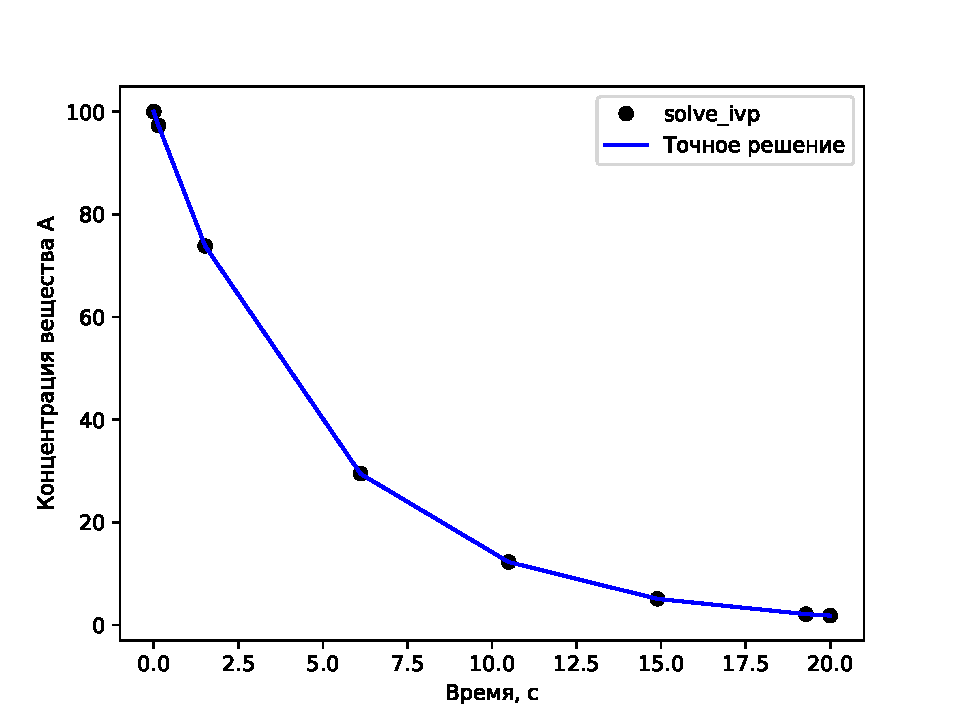
\includegraphics[width=\linewidth]{./pics/Figure_34}
	\caption{Снижение концентрации реагента в реакции первого порядка: аналитическое и численное решения}
\end{figure}
\end{minipage}
\begin{minipage}{.4\linewidth}
	\begin{itemize}
		\item Данный подход оправдан в тех случаях, когда требуется определить только конечную концентрацию реагента, однако для отслеживания изменения концентрации во времени с более высокой дискретностью можно передать специальную последовательность точек по времени в опциональном аргументе \texttt{t\_eval}.
	\end{itemize}
\end{minipage}
\vfill
\end{frame}

\begin{frame}[fragile, label=c]{Обыкновенные дифференциальные уравнения}
\scriptsize
\begin{itemize}
	\item Разобьем наш интервал интегрирования на 20 точек по времени:
\vfill
\begin{minted}{pycon}
>>> t0, tf = 0, 20
>>> t_eval = np.linspace(t0, tf, 20)
>>> solution = solve_ivp(func, (t0, tf), [y0], t_eval=t_eval)
>>> t, y = solution.t, solution.y[0]
\end{minted}
\vfill
	\item В опциональный  аргумент \mintinline{python}|dense_output| можно передать значение \mintinline{python}|True| для определения объекта \mintinline{python}|OdeSolution| с атрибутом \mintinline{python}|sol| как одним из возвращаемых объектов.
	\item Данный функционал можно использовать для генерации значений решения в промежуточных точках по времени:
\vfill
\begin{minted}{pycon}
>>> # Начальная и конечные точки по времени интегрирования
>>> t0, tf = 0, 20
>>> # Интегрирования дифференциального уравнения
>>> solution = solve_ivp(func, (t0, tf), [y0], dense_output=True)
>>> t = np.linspace(t0, tf, 20)
>>> y = solution.sol(t)[0]
\end{minted}
\vfill
	\item Объект \texttt{solution.sol} можно вызывать: значение независимой переменной~-- времени~-- передается в него как аргумент, и возвращается массив решений в этот момент времени. В рассмотренном случае есть только одна зависимая переменная \texttt{y}, поэтому используется индекс \texttt{[0]}.
\end{itemize}
\vfill
\end{frame}

\begin{frame}[fragile, label=c]{Обыкновенные дифференциальные уравнения}
\scriptsize
\begin{minipage}{.58\textwidth}
\begin{figure}[h!]
	\centering
	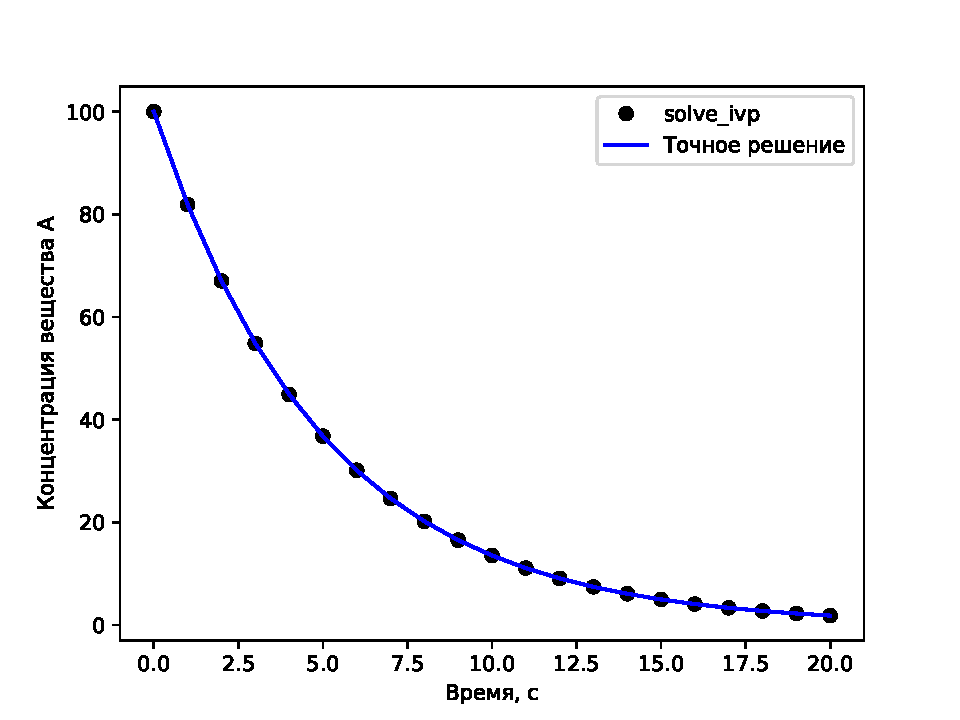
\includegraphics[width=.92\linewidth]{./pics/Figure_35}
	\caption{Снижение концентрации реагента по времени: аналитическое и численное решение с использованием предварительно определенных точек}
\end{figure}
\end{minipage}
\begin{minipage}{.415\textwidth}
\begin{itemize}
	\item Аналогично методу \texttt{quad}, дополнительные аргументы можно передать через параметр \texttt{args}.
	\item В рассмотренном выше примере константа скорости реакции \texttt{k} определена в глобальной области видимости, однако лучше передавать эту переменную явным образом:

\begin{minted}[frame=none]{pycon}
>>> def func(t, y, k):
...     return -k * y
...
\end{minted}
\end{itemize}
\end{minipage}
\begin{itemize}
	\item Дополнительные аргументы указываются в параметре \texttt{args}:
\vfill
\begin{minted}[frame=none]{pycon}
>>> solution = solve_ivp(func, (t0, tf), [y0], args=(k,))
\end{minted}
\end{itemize}
\vfill
\end{frame}

%\subsubsection{Система взаимосвязанных ОДУ первого порядка}
\begin{frame}[fragile, label=c]{Система взаимосвязанных ОДУ первого порядка}
\scriptsize
\textcolor{tpugreen}{\textbf{Решение системы ОДУ первого порядка}}
\vfill
	Метод \texttt{solve\_ivp} также может быть использован для решения системы взаимосвязанных ОДУ первого порядка с несколькими зависимыми переменными $y_1(t), y_2(t),\dots, y_n(t)$:
\vfill
\begin{equation*}
	\left\{
	\begin{aligned}
		\dfrac{dy_1}{dt} &= f_1\left(y_1, y_2,\dots, y_n; t\right)\\
		\dfrac{dy_2}{dt} &= f_2\left(y_1, y_2,\dots, y_n; t\right)\\
		\dots \\
		\dfrac{dy_n}{dt} &= f_n\left(y_1, y_2,\dots, y_n; t\right)
	\end{aligned}
	\right.
\end{equation*}
\vfill
\begin{minted}{pycon}
>>> def func(t, y):
...     # y = [y1, y2, ... yn] - последовательность зависимых переменных
...     dy1dt = f1(y, t)
...     dy2dt = f2(y, t)
...     # ... и т.д.
...     # Возвращаются вычисленные производные в последовательности,
...     # например, в кортеже
...     return dy1dt, dy2dt, ... dyndt
\end{minted}
\vfil
\end{frame}

\begin{frame}[fragile, label=c]{Система взаимосвязанных ОДУ первого порядка}
\scriptsize
Для наглядной демонстрации рассмотрим следующую схему химических реакций:
\vfill
$$
	A \rightarrow B \rightarrow C
$$
\vfill
\noindent с константами скоростей $k_1$ и $k_2$. Уравнения, описывающие скорость изменения концентраций компонентов по времени, записываются следующим образом:
\vfill
\begin{equation*}
	\left\{
	\begin{aligned}
		\dfrac{d\left[A\right]}{dt} &= -k_1\left[A\right] \\
		\dfrac{d\left[B\right]}{dt} &=  k_1\left[A\right] - k_2\left[B\right] \\
		\dfrac{d\left[C\right]}{dt} &=  k_2\left[B\right] \\
	\end{aligned}
	\right.
\end{equation*}
\vfill
Для численного решения предположим $y_1 \equiv \left[A\right]$,  $y_2 \equiv \left[B\right]$ и $y_3 \equiv \left[C\right]$:
\vfill
\begin{equation*}
	\left\{
	\begin{aligned}
		\dfrac{d\left[A\right]}{dt} &= -k_1y_1 \\
		\dfrac{d\left[B\right]}{dt} &=  k_1y_1 - k_2y_2 \\
		\dfrac{d\left[C\right]}{dt} &=  k_2y_2 \\
	\end{aligned}
	\right.
\end{equation*}
\vfill
\end{frame}

\begin{frame}[fragile, label=c]{Система взаимосвязанных ОДУ первого порядка}
\scriptsize
Зададимся значениями констант: $k_1 = 0.2 \text{ } c^{-1}$, $k_2 = 0.8 \text{ } c^{-1}$ и начальными условиями: $y_1(0) = 100$, $y_2(0) = 0$ $y_3(0) = 0$.
\vfill
\begin{minted}{pycon}
>>> import numpy as np
>>> from scipy.integrate import solve_ivp
>>> # константы скоростей и начальные условия
>>> k1, k2 = 0.2, 0.8
>>> a0, b0, c0 = 100, 0, 0
>>> t0, tf = 0, 20
>>> def func(t, y, k1, k2):
...     """"Returns dy_i/dt = f(t, y_i) at time t."""
...     y1, y2, y3 = y
...     dy1dt = -k1 * y1
...     dy2dt = k1 * y1 - k2 * y2
...     dy3dt = k2 * y2
...     return dy1dt, dy2dt, dy3dt
...
>>> y0 = a0, b0, c0
\end{minted}
\vfill
\end{frame}

\begin{frame}[fragile, label=c]{Система взаимосвязанных ОДУ первого порядка}
\scriptsize
\begin{minted}{pycon}
>>> solution = solve_ivp(func, (t0, tf), y0, dense_output=True, args=(k1, k2))
>>> t = np.linspace(t0, tf, 50)
>>> a, b, c = solution.sol(t)
>>> # аналитическое решение
>>> a_exact = a0 * np.exp(-k1 * t)
>>> b_exact = a0 * k1 / (k2 - k1) * (np.exp(-k1 * t) - np.exp(-k2 * t))
>>> c_exact = a0 - a_exact - b_exact
\end{minted}
\vfill
\end{frame}

\begin{frame}[fragile, label=c]{Система взаимосвязанных ОДУ первого порядка}
\scriptsize
\begin{figure}[h!]
	\centering
	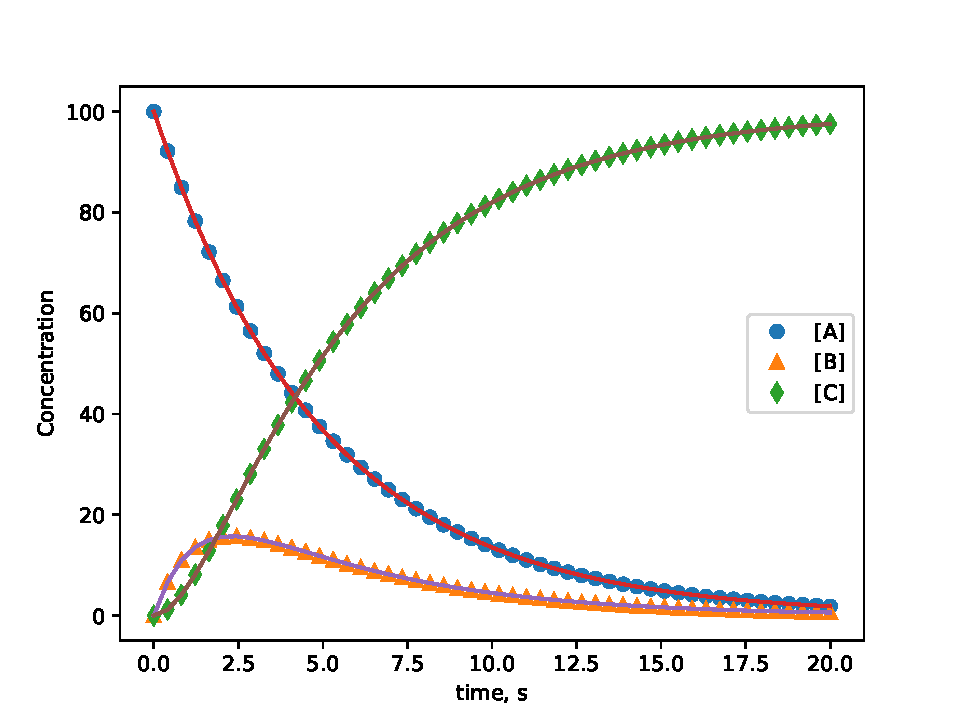
\includegraphics[width=.65\linewidth]{./pics/Figure_36}
	\caption{Схема из двух взаимосвязанных химических реакций первого порядка: численное и аналитическое решения}
\end{figure}
\vfill
\end{frame}

\section{Интерполяция и аппроксимация}
\sectionframe

\subsection{Одномерная интерполяция}
\begin{frame}[fragile, label=c]{Одномерная интерполяция}
\scriptsize
\begin{itemize}
	\item Метод \texttt{scipy.interpolate.interp1d} представляет метод одномерной интерполяции.
	\item Данный метод в качестве входных параметров принимает массивы точек \texttt{x} и \texttt{y}, а возвращает объект функции, который можно вызывать для получения интерполируемых значений в промежуточных точках \texttt{x}.
	\item По умолчанию используется линейная схема интерполяции, однако существует возможность применения и других вариантов.
\end{itemize}
\vfill
\begin{table}[h!]
%	\caption{Схемы интерполяции, передаваемые в аргументе \texttt{kind} при вызове метода \texttt{scipy.interpolate.interp1d}}
%	\label{tab:interp1d}
	\begin{tabular*}{\linewidth}{p{0.15\linewidth}p{0.8\linewidth}}
		\hline
		\textbf{\texttt{kind} }& \textbf{Описание} \\
		\hline
		\mintinline{python}|'linear'| & Принятая по умолчанию линейная интерполяция, использующая при расчетах только значения из исходных данных, охватывающих требуемую точку \\
		\mintinline{python}|'nearest'| & Привязка к ближайшей	 точке данных \\
		\mintinline{python}|'zero'| & Сплайн нулевого порядка: интерполирует по последнему наблюдаемому значению при проходе по массиву данных \\
		\mintinline{python}|'slinear'| & Интерполяция сплайном первого порядка (аналог \mintinline{python}|'linear'|) \\
		\mintinline{python}|'quadratic'| & Интерполяция сплайном второго порядка \\
		\mintinline{python}|'cubic'| & Интерполяция кубическим сплайном \\
		\mintinline{python}|'previous'| & Используется предыдущая точка данных \\
		\hline
	\end{tabular*}
\end{table}
\vfill
\end{frame}

\begin{frame}[fragile, label=c]{Одномерная интерполяция}
\scriptsize
\begin{minted}{pycon}
>>> import numpy as np
>>> from scipy.interpolate import interp1d
>>> a, nu, k = 10, 4, 2
>>> def func(x, a, nu, k):
...     return a * np.exp(-k * x) * np.cos(2 * np.pi * nu * x)
...
>>> xmax, nx = 0.5, 8
>>> x = np.linspace(0, xmax, nx)
>>> y = func(x, a, nu, k)
>>> nearest = interp1d(x, y, kind='nearest')
>>> linear = interp1d(x, y)
>>> cubic = interp1d(x, y, kind='cubic')
\end{minted}
\vfill
\end{frame}

\begin{frame}[fragile, label=c]{Одномерная интерполяция}
\scriptsize
\begin{figure}[h!]
	\centering
	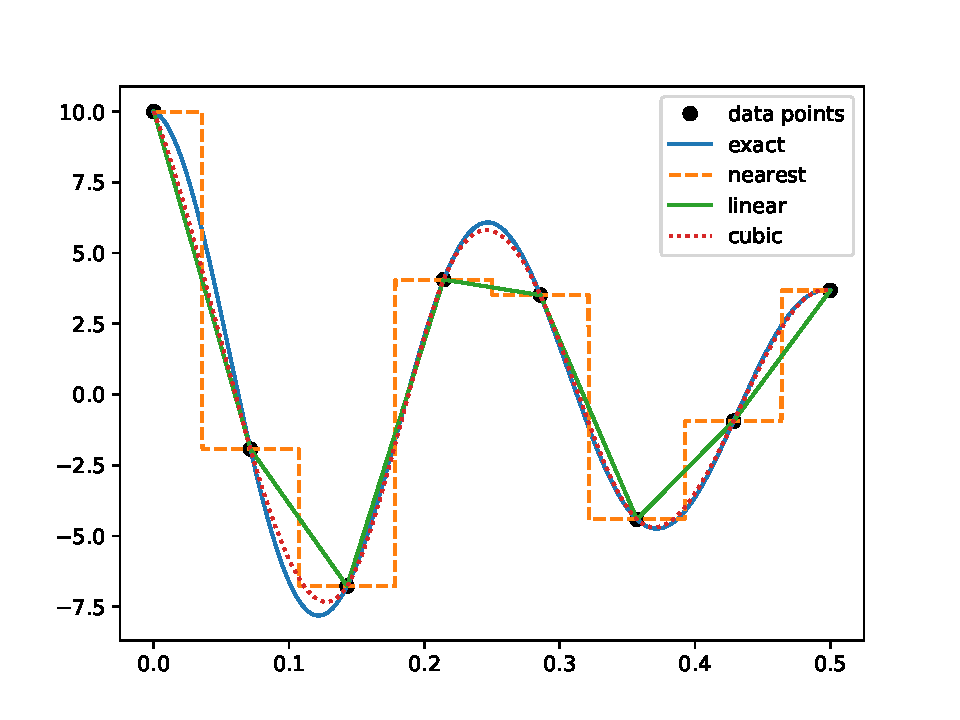
\includegraphics[width=.65\linewidth]{./pics/Figure_37}
	\caption{Демонстрация различных методик интерполяции, доступных в методе \texttt{scipy.interpolate.interp1d}}
\end{figure}
\vfill
\end{frame}

\subsection{Нелинейная аппроксимация методом \\ наименьших квадратов}
\begin{frame}[fragile, label=c]{Нелинейная аппроксимация методом \\ наименьших квадратов}
\scriptsize
В библиотеке SciPy реализована нелинейная аппроксимация методом наименьших квадратов в виде  \texttt{scipy.optimize.leastsq}. Базовая сигнатура вызова данного метода выглядит следующим образом:
\vfill
\begin{minted}[frame=none]{pycon}
>>> scipy.optimize.leastsq(func, x0, args=())
\end{minted}
\vfill
\begin{itemize}
	\item Данный метод выполняет аппроксимацию последовательности точек данных \texttt{y} моделируемой функцией \texttt{f}, зависящей от одного или нескольких параметров аппроксимации.
	\item В функцию \texttt{leastsq} необходимо передать соответствующий объект функции \texttt{func}, которая возвращает разность между \texttt{y} и \texttt{f} (остатки).
	\item Также необходимо задать начальное приближение для \texttt{x0}.
	\item Если функция \texttt{func} требует дополнительные аргументы, то их можно передать в кортеже \texttt{args}.
	Для наглядности рассмотрим аппроксимацию искусственно зашумленной функции затухающего косинуса
\vfill
$$
	f(t) = ae^{-t/\tau}\cos2\pi\nu t
$$
\end{itemize}
\vfill
\end{frame}

\begin{frame}[fragile, label=c]{Нелинейная аппроксимация методом \\ наименьших квадратов}
\scriptsize
\begin{minted}{pycon}
>>> import numpy as np
>>> a, freq, tau = 10, 4, 0.5
>>> def f(t, a, freq, tau):
...     return a * np.exp(-t / tau) * np.cos(2 * np.pi * freq * t)
...
>>> tmax, dt = 1, 0.01
>>> t = np.arange(0, tmax, dt)
>>> y_exact = f(t, a, freq, tau)
>>> y = y_exact + np.random.randn(y_exact.shape[0]) * 2
\end{minted}
\vfill
\end{frame}

\begin{frame}[fragile, label=c]{Нелинейная аппроксимация методом \\ наименьших квадратов}
\scriptsize
\begin{figure}[h!]
	\centering
	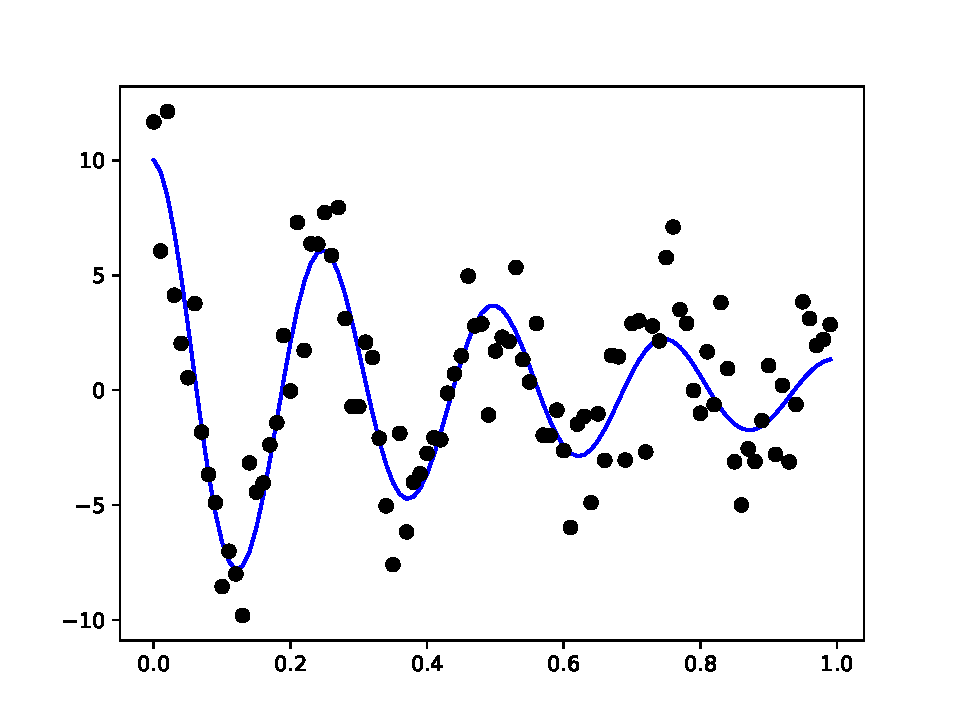
\includegraphics[width=.6\linewidth]{./pics/Figure_38}
	\caption{Функция затухающего косинуса с искусственным зашумлением}
\end{figure}
\vfill
\end{frame}

\begin{frame}[fragile, label=c]{Нелинейная аппроксимация методом \\ наименьших квадратов}
\scriptsize
Задача аппроксимации зашумленного набора данных сводится к определению параметров \texttt{a}, \texttt{freq} и \texttt{tau} (представим, что они нам неизвестны).
\vfill
\begin{itemize}
	\item Для решения этой задачи сначала необходимо определить функцию \texttt{residuals}:
\vfill
\begin{minted}{pycon}
>>> def residuals(params, y, t):
...     a, freq, tau = params
...     return y - f(t, a, freq, tau)
...
\end{minted}
\vfill
	\item Первый аргумент~-- последовательность параметров \texttt{params} которые для лучшей читаемости кода распаковываются в именованные переменные.
	\item Требуемые дополнительные аргументы: набор точек данных \texttt{y} и независимая переменная \texttt{t}.
	\item Далее необходимо задать начальные приближения для параметров и вызвать метод \texttt{leastsq}:
\vfill
\begin{minted}{pycon}
>>> from scipy.optimize import leastsq
>>> params0 = 5, 5, 1
>>> plsq = leastsq(residuals, params0, args=(y, t))
>>> plsq[0]
array([9.1920154, 4.0158567, 0.593839 ])
\end{minted}
\end{itemize}
\vfill
Действительные значения параметров \texttt{a, freq, tau = 10, 4, 0.5}, таким образом, учитывая шум, добавленный к исходным данным, результат можно считать вполне приемлемым.
\vfill
\end{frame}

\begin{frame}[fragile, label=c]{Нелинейная аппроксимация методом \\ наименьших квадратов}
\scriptsize
\begin{figure}[h!]
	\centering
	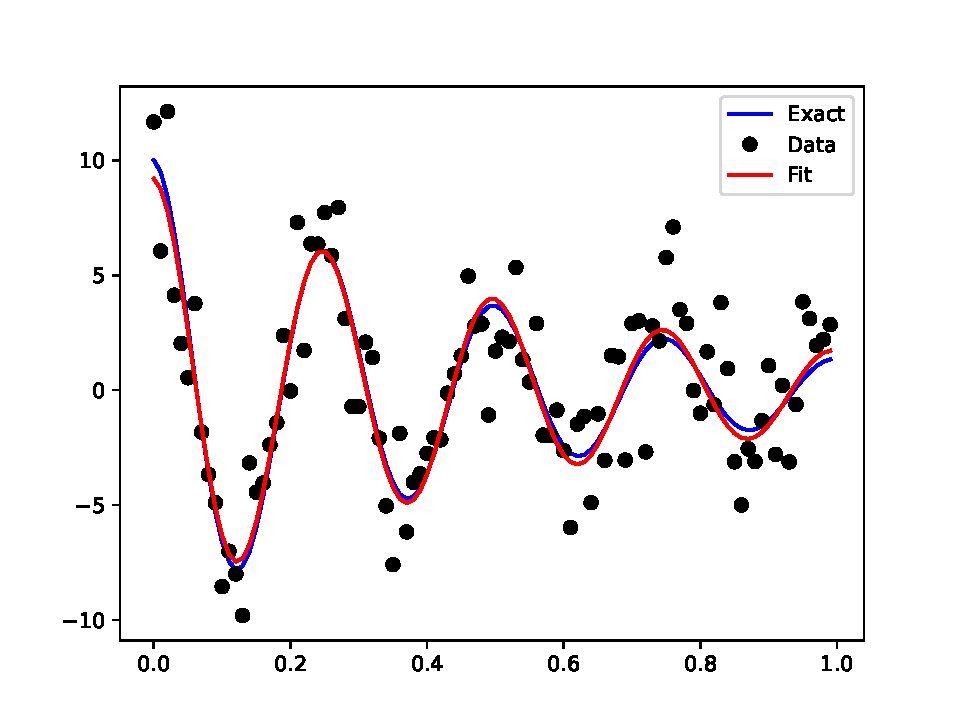
\includegraphics[width=.6\textwidth]{./pics/Figure_39.pdf}
	\caption{Нелинейная аппроксимация методом наименьших квадратов для функции затухающего косинуса с зашумлением}
	\label{fig:figure_39}
\end{figure}
\vfill
\end{frame}

\begin{frame}[fragile]{Аппроксимация}
\scriptsize
Дана табличная зависимость энтропии вещества от температуры.
\begin{table}[h!]
	\centering
	\begin{tabular}{|l|r|r|r|r|r|}
		\hline
		$T$, K & $298.15$ & $400$ & $500$ & $600$ & $700$ \\
		\hline
		$S,\ \mathrm{Дж/(моль \cdot K)}$ & $49.15$ & $51.36$ & $53.30$ & $54.97$ & $56.40$ \\
		\hline
	\end{tabular}
\end{table}
Необходимо построить линейную, степенную и экспоненциальную аппроксимирующие функции и найти значение теплоемкости при температуре $T=650$ K.
\vfill
\begin{itemize}
\item Линейная функция:
$$
	y = a_0 + a_1 \cdot x
$$
где $a_0$ и $a_1$~-- коэффициенты.
\item Степенная функция:
$$
	y = a \cdot x ^ b
$$
где $a$ и $b$~-- коэффициенты.
\item Экспоненциальная функция:
$$
	y = a \cdot e^ {b \cdot x}
$$
где $a$ и $b$~-- коэффициенты.
\end{itemize}
\vfill
\end{frame}


\begin{frame}[fragile]{Аппроксимация}
\scriptsize
\begin{minted}[escapeinside=&&]{python}
from __future__ import annotations  # для версии Python ниже 3.10
import numpy as np
from typing import Callable
from scipy.optimize import least_squares


def linear(x: float | np.ndarray,
           params: tuple[float, float]) -> float | np.ndarray:
    a0, a1 = params
    return a0 + a1 * x

def power(x: float | np.ndarray,
          params: tuple[float, float]) -> float | np.ndarray:
    a, b = params
    return a * x ** b

def exponent(x: float | np.ndarray,
             params: tuple[float, float]) -> float | np.ndarray:
    a, b = params
    return a * np.exp(b * x)
&\space&
\end{minted}
\vfill
\end{frame}


\begin{frame}[fragile]{Аппроксимация}
\scriptsize
\begin{minted}[firstnumber=last]{python}
def residuals(params: tuple[float, float], x: np.ndarray,
              y: np.ndarray, func: Callable) -> np.ndarray:
    return y - func(x, params)


t = np.array([298.15, 400, 500, 600, 700])
s = np.array([49.15, 51.36, 53.30, 54.97, 56.40])
t_new = 650
x0 = 0.01, 0.01

results = least_squares(residuals, x0=x0, args=(t, s, linear))
linear_params, linear_cost = results.x, results.cost
print(linear_params, linear_cost)

results = least_squares(residuals, x0=x0, args=(t, s, power))
power_params, power_cost = results.x, results.cost
print(power_params, power_cost)

results = least_squares(residuals, x0=x0, args=(t, s, exponent))
exponent_params, exponent_cost = results.x, results.cost
print(exponent_params, exponent_cost)
\end{minted}
\vfill
\end{frame}

\begin{frame}[fragile]{Аппроксимация}
\scriptsize
Результаты расчетов:
\begin{itemize}
\item Линейная аппроксимация
\begin{minted}{pycon}
[4.40187563e+01 1.80478428e-02] 0.11106445922161706
\end{minted}
\item Степенная аппроксимация
\begin{minted}{pycon}
[19.46645965  0.16224222] 0.011577630390983832
\end{minted}
\item Экспоненциальная аппроксимация
\begin{minted}{pycon}
[4.47183499e+01 3.39118322e-04] 0.17227508882258857
\end{minted}
\end{itemize}
\vfill
Суммарная ошибка для степенной аппроксимации минимальна, поэтому выбираем данный вид функции для определения энтропии:
\vfill
\begin{minted}{python}
s_new = power(t_new, power_params)
print(s_new)
|\space|
\end{minted}
\begin{minted}{pycon}
55.67500745784808
\end{minted}
\vfill
\end{frame}

\section{Численные методы решения уравнений}
\sectionframe

\begin{frame}[fragile, label=c]{Численные методы решения уравнений}
\scriptsize
Модуль \texttt{scipy.optimize} содержит несколько методов для определения корней уравнений с одной или несколькими неизвестными величинами: \texttt{brentq, brenth, ridder, bisect}.
\vfill
\begin{itemize}
\item Каждый из указанных выше методов требует непрерывную функцию $f(x)$ и пару чисел, определяющих интервал поиска корней, т.е. значения \texttt{a} и \texttt{b}, такие, что корень находится в интервале $[a, b]$ и $f(a) \cdot f(b) < 0$.
\item Наиболее распространенным методом поиска корней функции является \texttt{scipy.optimize.brentq}, являющийся реализацией метода Брента с обратной квадратичной экстраполяцией (\texttt{scipy.optimize.brenth}~-- аналогичный метод, использующий гиперболическую экстраполяцию). Рассмотрим в качестве демонстрации следующую функцию на интервале ${-1 \leqslant x \leqslant 1}$:
\vfill
$$
	f(x) = \dfrac{1}{5} +  x\cos\left(\dfrac{3}{x}\right)
$$
\vfill
\item  График этой функции (рисунок~\ref{fig:figure_41}) показывает, что корень находится между $\mathrm{-}0.7$ и $\mathrm{-}0.5$.
\end{itemize}
\vfill
\end{frame}

\begin{frame}[fragile, label=c]{Численные методы решения уравнений}
\scriptsize
\begin{minipage}{.55\textwidth}
\begin{figure}[h!]
 	\centering
 	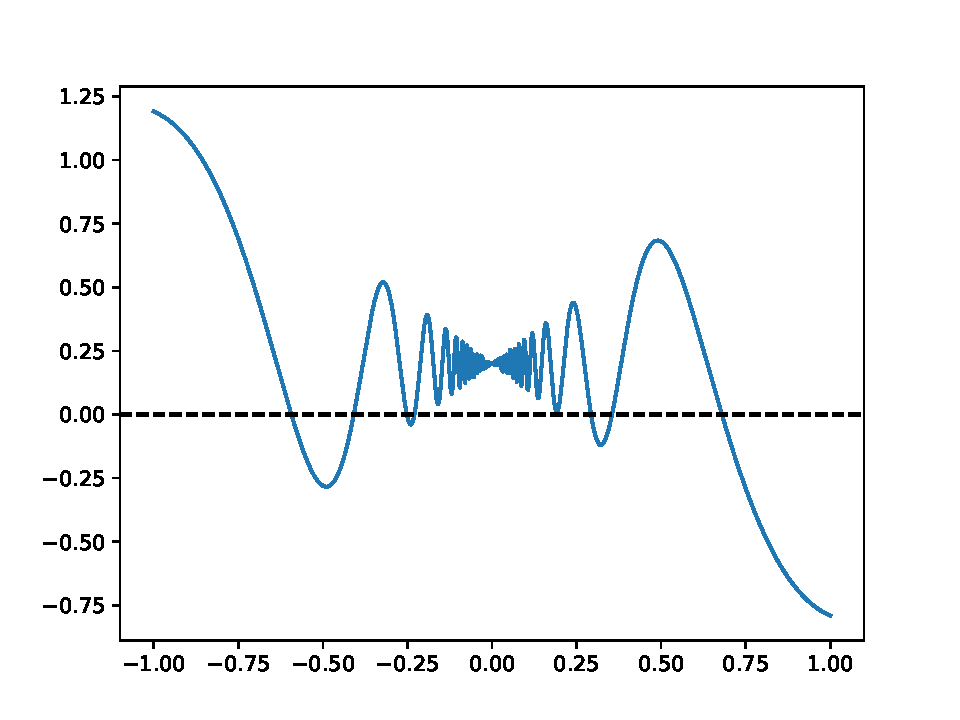
\includegraphics[width=\linewidth]{./pics/Figure_41}
 	\caption{График функции $f(x) = 1/5 + x\cos\left(3/x\right)$}
 	\label{fig:figure_41}
 \end{figure}
\end{minipage}
\begin{minipage}{.03\textwidth}
\hfill
\end{minipage}
\begin{minipage}{.3\textwidth}
\begin{minted}{python}
import numpy as np
import scipy.optimize as opt


def f(x: float) -> float:
    return 1 / 5 + x * np.cos(3 / x)


root = opt.brentq(f, -.7, -.5)
print(root)
|\space|
\end{minted}
\begin{minted}[frame=none]{pycon}
-0.5933306271014237
\end{minted}
\end{minipage}
\vfill
\end{frame}

\begin{frame}[fragile, label=c]{Численные методы решения уравнений}
\scriptsize
\begin{itemize}
\item Метод Риддерса для поиска корней функции реализован в библиотеке SciPy как метод \texttt{scipy.optimize.ridder}.
\item Наиболее медленный, но весьма надежный \textcolor{tpugreen}{\textbf{метод бисекций}} реализован в \texttt{scipy.optimize.bisect}.
\item Одним из быстрейших методов поиска корней является алгоритм Ньютона-Рафсона в тех случаях, когда можно найти определить первую производную $f^{\ \prime}(x)$.
\item В тех случаях, когда возможно написать исходный код для аналитического выражения первой производной $f^{\ \prime}(x)$, этот код передается в метод \texttt{scipy.optimize.newton} в виде аргумента \texttt{fprime} вместе с начальной точкой \texttt{x0}, которая должна находится как можно ближе к определяемому корню. В данном случае нет необходимости определять ограничивающий интервал для поиска корня.
\item Если первую производную $f^{\ \prime}(x)$ выразить аналитически невозможно, то в методе \texttt{newton} используется \textcolor{extraorange}{\textbf{алгоритм секущих}}.
\end{itemize}
\vfill
\end{frame}


\section{Визуализация данных с \\ помощью библиотеки Matplotlib}
\sectionframe

\begin{frame}[fragile, label=m]{Библиотека Matplotlib}
\scriptsize
\begin{minipage}{.85\textwidth}
\begin{itemize}
\item \textbf{Matplotlib}~-- библиотека для визуализации данных, основанная на массивах  \texttt{NumPy}.
\item Важнейшей возможностью данного пакета является хорошая совместимость с множеством операционных систем и графических прикладных частей.
\end{itemize}
\end{minipage}
\begin{minipage}{.14\textwidth}

\includegraphics[width=\linewidth]{./pics/mpl_logo}
\end{minipage}
\begin{itemize}
\item Полезным источником информации является галерея Matplotlib (\url{https://matplotlib.org/stable/gallery/index.html}). Галерея содержит большое количество миниатюр различных типов графиков, каждая из которых является ссылкой на страницу с фрагментом кода на языке Python, используемым для его генерации.
\end{itemize}
\vfill
Для импорта библиотеки Matplotlib приняты стандартные сокращения:
\vfill
\begin{minted}{pycon}
>>> import matplotlib as mpl
>>> import matplotlib.pyplot as plt
\end{minted}
\vfill
Используемая версия библиотеки - 3.8.2
\vfill
\end{frame}

\begin{frame}[fragile, label=m]{Настройка стилей}
\scriptsize
Для того чтобы настроить стиль графиков, будем использовать команду \texttt{plt.style}. Ниже приведен пример выбора стиля \texttt{classic}, который обеспечит в создаваемых  графиках классический стиль библиотеки Matplotlib:
\vfill
\begin{minted}{pycon}
>>> import matplotlib.pyplot as plt
>>> plt.style.use('classic')
\end{minted}
\vfill
Для того, чтобы увидеть список доступных для использования стилей, необходимо выполнить следующую инструкцию:
\begin{minted}{pycon}
>>> plt.style.available
['Solarize_Light2', '_classic_test_patch', '_mpl-gallery', '_mpl-gallery-nogrid', 'bmh',
'classic', 'dark_background', 'fast', 'fivethirtyeight', 'ggplot', 'grayscale',
 'seaborn-v0_8', 'seaborn-v0_8-bright', 'seaborn-v0_8-colorblind', 'seaborn-v0_8-dark',
 'seaborn-v0_8-dark-palette', 'seaborn-v0_8-darkgrid', 'seaborn-v0_8-deep',
 'seaborn-v0_8-muted', 'seaborn-v0_8-notebook', 'seaborn-v0_8-paper', 'seaborn-v0_8-pastel',
 'seaborn-v0_8-poster', 'seaborn-v0_8-talk', 'seaborn-v0_8-ticks', 'seaborn-v0_8-white',
 'seaborn-v0_8-whitegrid', 'tableau-colorblind10']
\end{minted}
\vfill
\end{frame}

\begin{frame}[fragile, label=m]{Построение графиков}
\scriptsize
Построение линейного графика можно выполнить при помощи следующих команд:
\vfill
\begin{minipage}{.4\textwidth}
\begin{minted}{python}
import numpy as np
import matplotlib.pyplot as plt


x = np.linspace(0, 10, 100)
plt.plot(x,  np.sin(x), '-')
plt.plot(x, np.cos(x), '--')
plt.show()
|\space|
\end{minted}
\end{minipage}
\begin{minipage}{.59\textwidth}
\begin{figure}[h!]
	\centering
	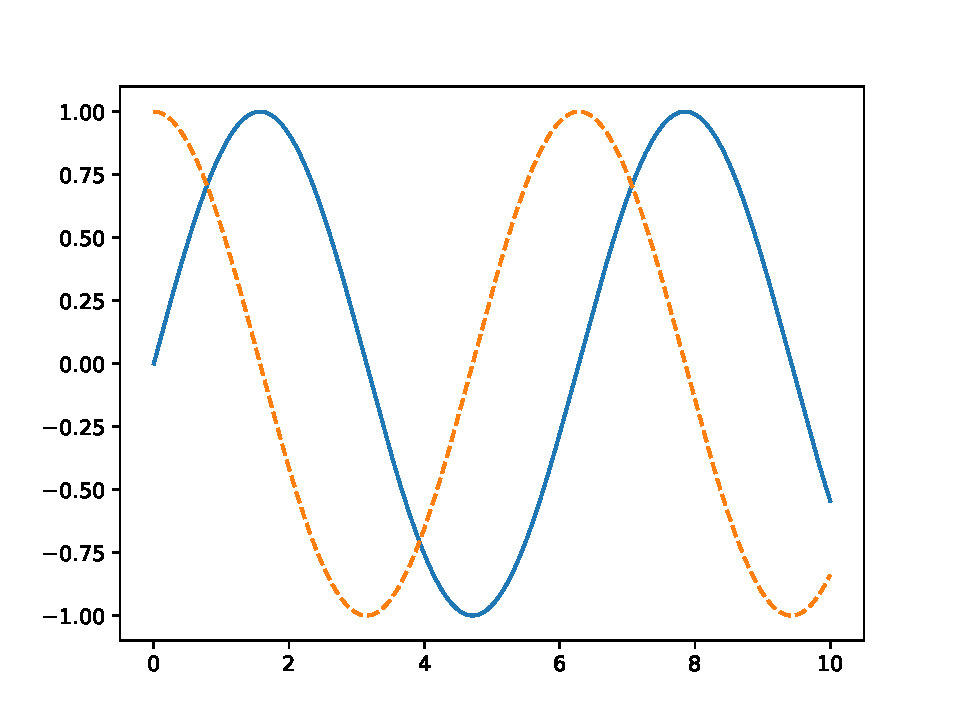
\includegraphics[width=\linewidth]{./pics/Figure_1.pdf}
	\caption{Пример построения графика}
\end{figure}
\end{minipage}
\vfill
\end{frame}

\begin{frame}[fragile, label=m]{Построение графиков}
\scriptsize
При необходимости совместить несколько графиков на одном рисунке можно воспользоваться функцией \mintinline{python}|subplots()|:
\vfill
\begin{minipage}{.38\textwidth}
\begin{minted}{python}
import numpy as np
import matplotlib.pyplot as plt


x = np.linspace(0, 10, 100)

fig, ax = plt.subplots(
    1, 2, figsize=(7, 3.)
)
ax[0].plot(x,  np.sin(x), '-')
ax[1].plot(x, np.cos(x), '--')

plt.show()
|\space|
\end{minted}
\end{minipage}
\begin{minipage}{.61\textwidth}
\begin{figure}[h!]
	\centering
	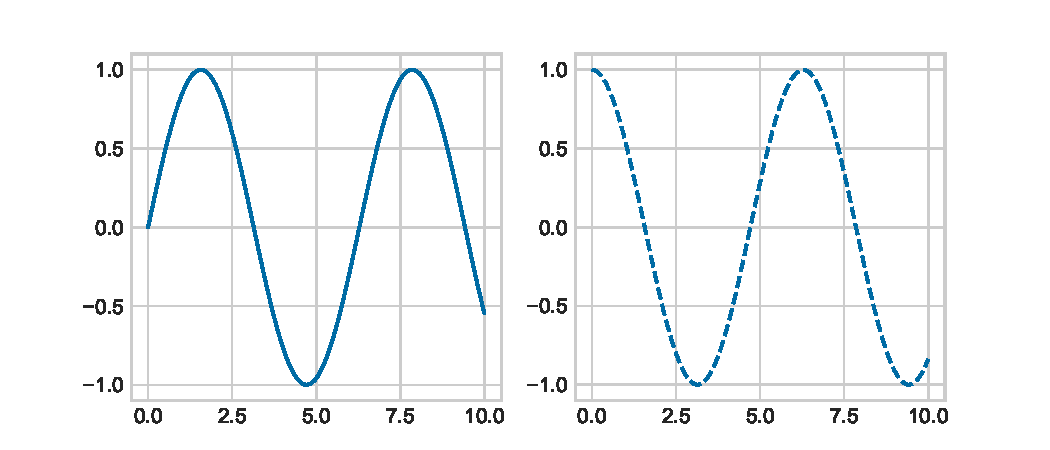
\includegraphics[width=1.1\linewidth]{./pics/double}
	\caption{Пример совмещения двух графиков на одном рисунке}
\end{figure}
\end{minipage}
\vfill
\end{frame}

\begin{frame}[fragile, label=m]{Сохранение рисунков}
\scriptsize
Библиотека Matplotlib предоставляет возможность сохранять рисунки в файлы различных форматов. К примеру, можно сохранить предыдущий рисунок в формате PNG:
\vfill
\begin{minted}[firstnumber=last]{python}
plt.savefig('myfig.png')
|\space|
\end{minted}
\vfill
Метод \texttt{savefig()} устанавливает формат файла, исходя из расширения в заданном пользователем имени файла. Список поддерживаемых форматов:
\vfill
\begin{minted}[firstnumber=last]{python}
plt.gcf().canvas.get_supported_filetypes()
|\space|
\end{minted}
\begin{minted}[frame=none]{pycon}
{'eps': 'Encapsulated Postscript',
 'jpg': 'Joint Photographic Experts Group',
 'jpeg': 'Joint Photographic Experts Group',
 'pdf': 'Portable Document Format',
 'pgf': 'PGF code for LaTeX',
 'png': 'Portable Network Graphics',
 'ps': 'Postscript',
 'raw': 'Raw RGBA bitmap',
 'rgba': 'Raw RGBA bitmap',
 'svg': 'Scalable Vector Graphics',
 'svgz': 'Scalable Vector Graphics',
 'tif': 'Tagged Image File Format',
 'tiff': 'Tagged Image File Format'}
\end{minted}
\vfill
\end{frame}

\begin{frame}[fragile, label=m]{Простые линейные графики}
\scriptsize
Рассмотрим построение графика визуализации отдельной функции $y = f(x)$, начав с импорта необходимых для этого модулей:
\vfill
\begin{minted}{python}
import numpy as np
import matplotlib.pyplot as plt
plt.style.use('seaborn-v0_8-whitegrid')
|\space|
\end{minted}
\vfill
Во все случаях в Matplotlib мы начинаем с создания рисунка и осей координат. В наиболее простом случае это можно выполнить следующим образом (рисунок \ref{fig:fig_3}):
\vfill
\begin{minted}[firstnumber=last]{python}
fig = plt.figure()
ax = plt.axes()
|\space|
\end{minted}
\vfill
\end{frame}

\begin{frame}[fragile, label=m]{Простые линейные графики}
\scriptsize
\begin{figure}[h!]
	\centering
	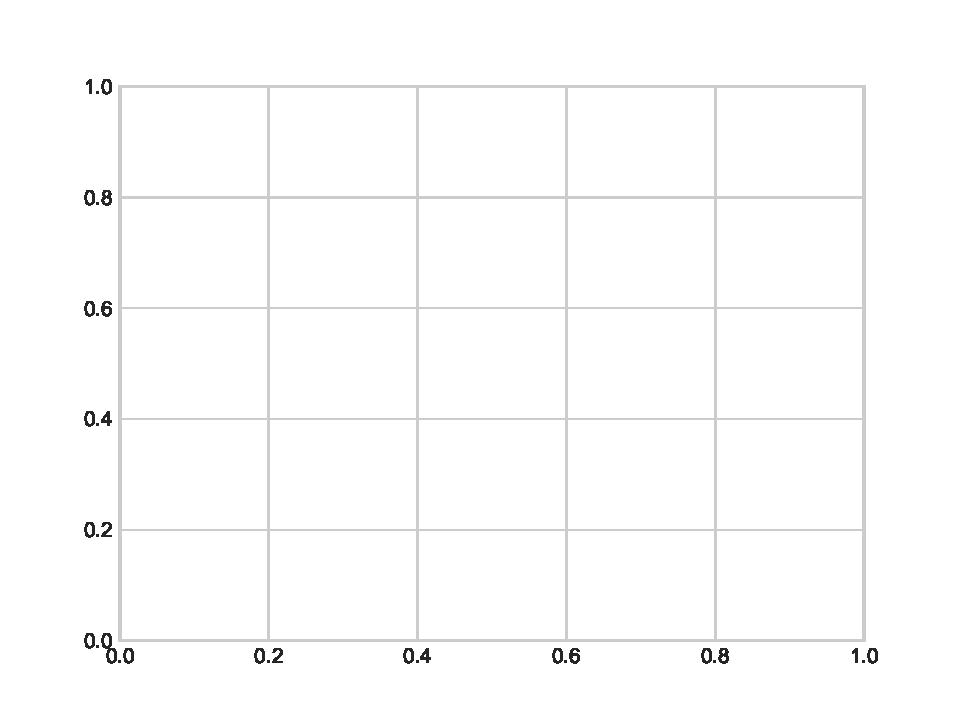
\includegraphics[width=0.6\linewidth]{./pics/Figure_3}
	\caption{Пустой рисунок с осями координат}
	\label{fig:fig_3}
\end{figure}
\vfill
\end{frame}

\begin{frame}[fragile, label=m]{Простые линейные графики}
\scriptsize
После того, как созданы оси, можно приступить к построению графика данных, применив метод \texttt{ax.plot(}). Рассмотрим простую синусоиду (рисунок~\ref{fig:fig_4}):
\vfill
\begin{minipage}{.4\textwidth}
\begin{minted}{python}
import numpy as np
import matplotlib.pyplot as plt


plt.style.use('seaborn-v0_8-whitegrid')

fig = plt.figure()
ax = plt.axes()

x = np.linspace(0, 10, 1000)
ax.plot(x, np.sin(x))

plt.show()
|\space|
\end{minted}
\end{minipage}
\begin{minipage}{.59\textwidth}
\begin{figure}[h!]
	\centering
	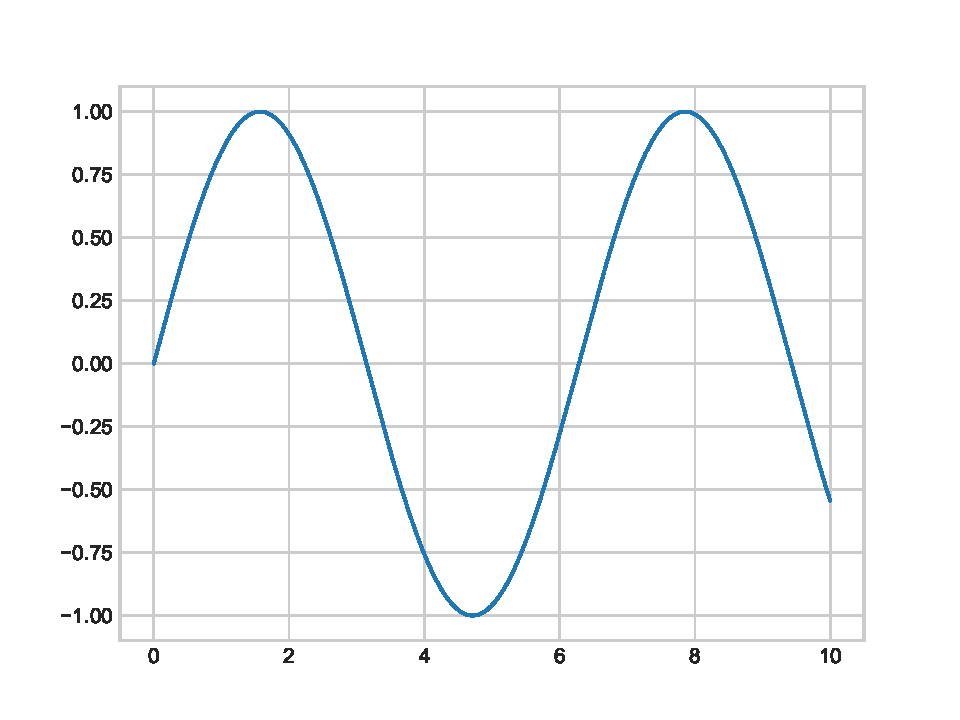
\includegraphics[width=\linewidth]{./pics/Figure_4.pdf}
	\caption{График простой синусоиды}
	\label{fig:fig_4}
\end{figure}
\end{minipage}
\vfill
\end{frame}


\begin{frame}[fragile, label=m]{Простые линейные графики}
\scriptsize
При необходимости создать рисунок с несколькими линиями, можно применить метод \texttt{plot} несколько раз, воспользовавшись объектно-ориентированным интерфейсом (рисунок~\ref{fig:fig_5}):
\vfill
\begin{minipage}{.4\textwidth}
\begin{minted}{python}
import numpy as np
import matplotlib.pyplot as plt


plt.style.use('seaborn-v0_8-whitegrid')

fig = plt.figure()
ax = plt.axes()

x = np.linspace(0, 10, 1000)
ax.plot(x, np.sin(x))
ax.plot(x, np.cos(x))

plt.show()
|\space|
\end{minted}
\end{minipage}
\begin{minipage}{.59\textwidth}
\begin{figure}[h!]
	\centering
	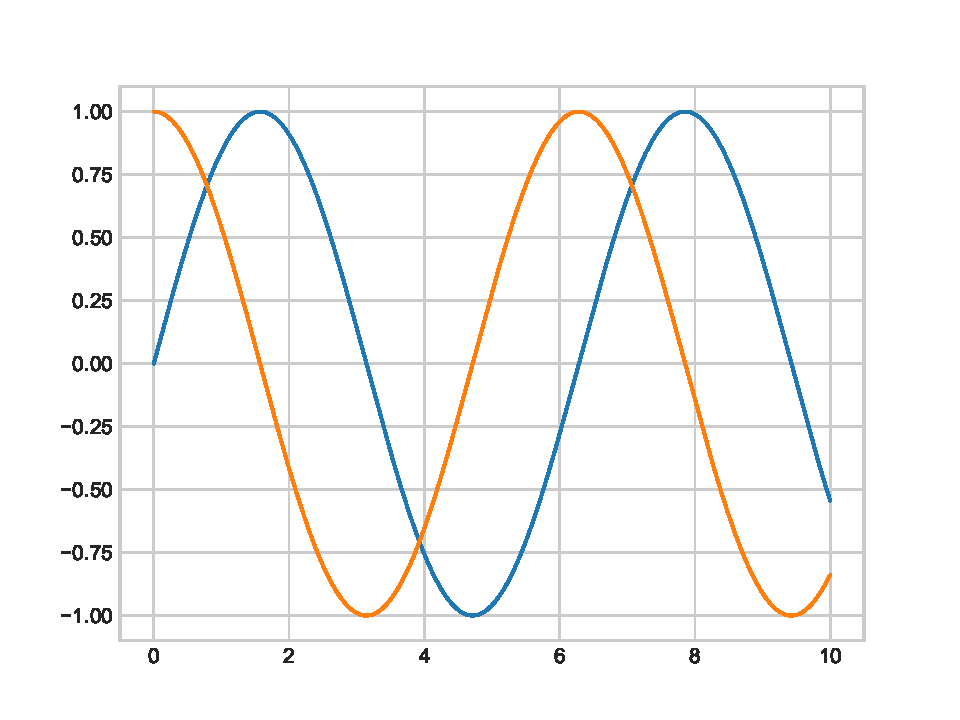
\includegraphics[width=\linewidth]{./pics/Figure_5.pdf}
	\caption{График с несколькими линиями}
	\label{fig:fig_5}
\end{figure}
\end{minipage}
\vfill
\end{frame}

\subsection{Настройка графика}
\begin{frame}[fragile, label=m]{Цвет и стиль линий}
\scriptsize
Функции \texttt{plt.plot} можно передавать дополнительные аргументы, позволяющие управлять цветами и стилями линий. Для настройки цвета используется ключевой слово \texttt{color} с соответствующим строковым аргументом, задающим почти любой цвет (рисунок~\ref{fig:fig_6}):
\vfill
\begin{minted}{python}
import numpy as np
import matplotlib.pyplot as plt

plt.style.use('seaborn-v0_8-whitegrid')
# цвет по названию
plt.plot(x, np.sin(x), color='blue')
# краткий код цвета (rgbcmyk)
plt.plot(x, np.sin(x - 1), color='g')
# Шкала оттенков серого цвета в диапазоне от 0 до 1
plt.plot(x, np.sin(x - 2), color='0.75')
# 16-ричный код (RRGGBB от 00 до FF)
plt.plot(x, np.sin(x - 3), color='#FFDD44')
# Кортеж RGB, значения от 0 до 1
plt.plot(x, np.sin(x - 4), color=(1.0, 0.2, 0.3))
# Поддерживаются все имена цветов HTML
plt.plot(x, np.sin(x - 5), color='chartreuse')

plt.show()
\end{minted}
\vfill
\end{frame}

\begin{frame}[fragile, label=m]{Цвет и стиль линий}
\scriptsize
\begin{figure}[h!]
	\centering
	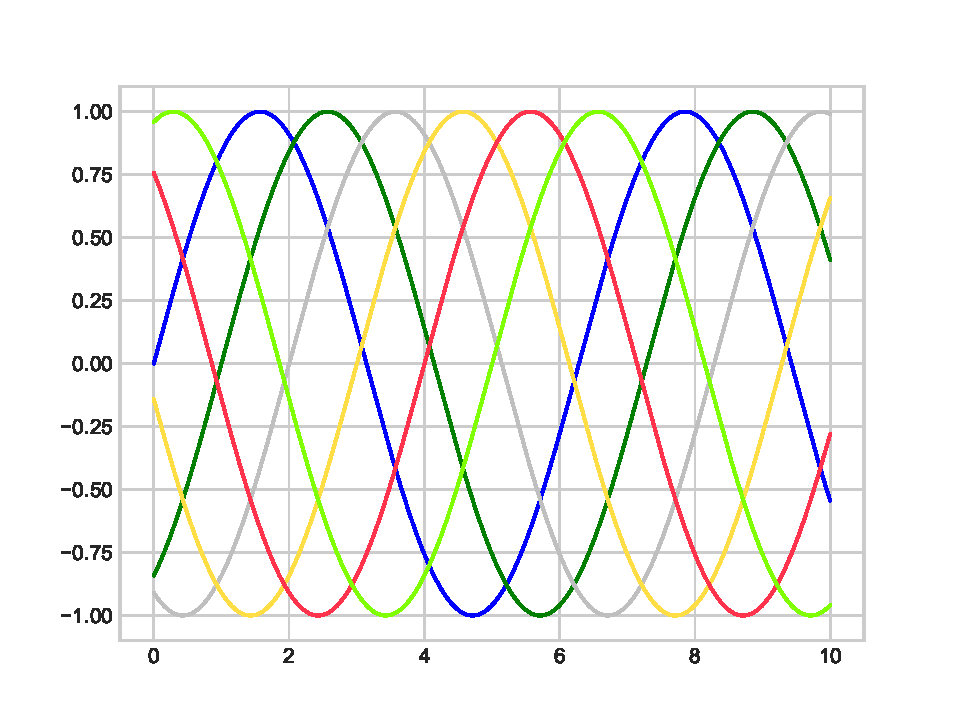
\includegraphics[width=.5\linewidth]{./pics/Figure_6}
	\caption{Настройка цвета линий графика}
	\label{fig:fig_6}
\end{figure}
\begin{itemize}
\item В том случае, если цвет не определен пользователем, выбор будет происходить автоматически по циклу из набора цветов по умолчанию, если график содержит несколько линий.
\end{itemize}
\vfill
\end{frame}

\begin{frame}[fragile, label=m]{Цвет и стиль линий}
\scriptsize
Стиль линий настраивается при помощи ключевого аргумента \texttt{linestyle} (рисунок \ref{fig:fig_7}):
\vfill
\begin{minted}{python}
import numpy as np
import matplotlib.pyplot as plt


plt.style.use('seaborn-v0_8-whitegrid')

plt.plot(x, x, linestyle='solid')
plt.plot(x, x + 1, linestyle='dashed')
plt.plot(x, x + 2, linestyle='dashdot')
plt.plot(x, x + 3, linestyle='dotted')
# разрешены следующие сокращения
plt.plot(x, x + 4, linestyle='-')  # сполшная
plt.plot(x, x + 5, linestyle='--') # штриховая
plt.plot(x, x + 6, linestyle='-.') # штрихпунктирная
plt.plot(x, x + 7, linestyle=':')  # линия из точек

plt.show()
|\space|
\end{minted}
\vfill
\end{frame}

\begin{frame}[fragile, label=m]{Цвет и стиль линий}
\scriptsize
\begin{figure}[h!]
	\centering
	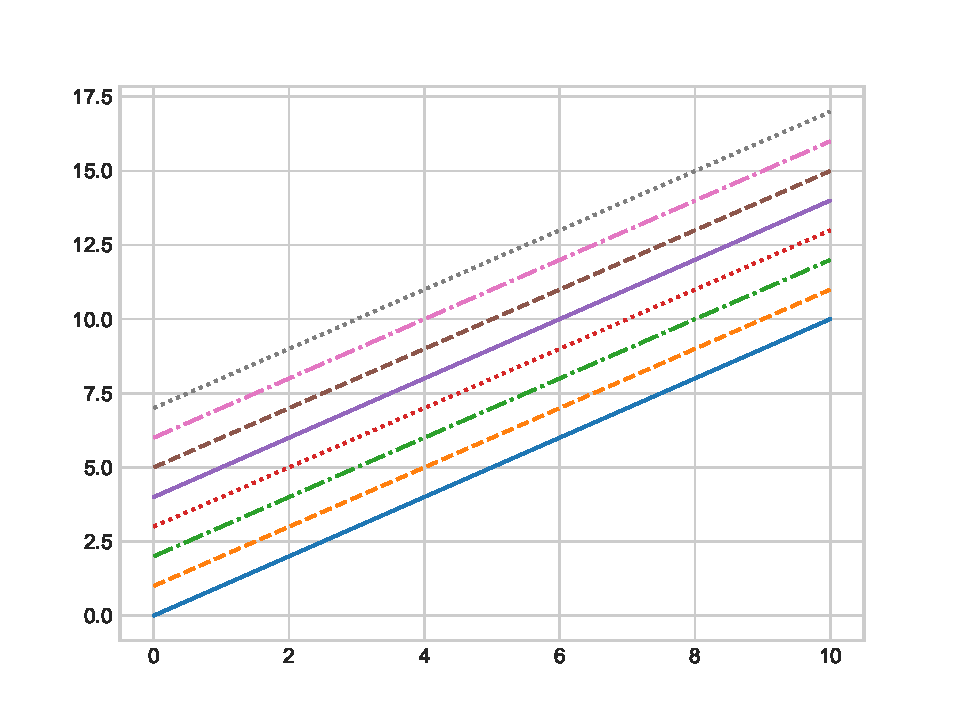
\includegraphics[width=.5\linewidth]{./pics/Figure_7}
	\caption{Настройка стиля линий графика}
	\label{fig:fig_7}
\end{figure}
\vfill
В действительности существует множество других аргументов для более тонкой настройки внешнего вида графика. Обратитесь к документации функции \texttt{plt.plot()} для более подробного изучения.
\vfill
\end{frame}

\subsection{Пределы осей координат}
\begin{frame}[fragile, label=m]{Пределы осей координат}
\scriptsize
В библиотеке Matplotlib достаточно хорошо реализован автоматический подбор пределов осей координат, однако в некоторых случаях требуется более тонкая настройка. Наиболее легкий путь~-- использовать методы \texttt{plt.xlim()} и \texttt{plt.ylim()} (рисунок~\ref{fig:fig_8}):
\vfill
\begin{minipage}{.4\textwidth}
\begin{minted}{python}
import numpy as np
import matplotlib.pyplot as plt


plt.style.use('seaborn-v0_8-whitegrid')

x = np.linspace(0, 10, 1000)
plt.plot(x, np.sin(x))
plt.xlim(-1, 11)
plt.ylim(-1.5, 1.5)

plt.show()
|\space|
\end{minted}
\end{minipage}
\begin{minipage}{.59\textwidth}
\begin{figure}[h!]
	\centering
	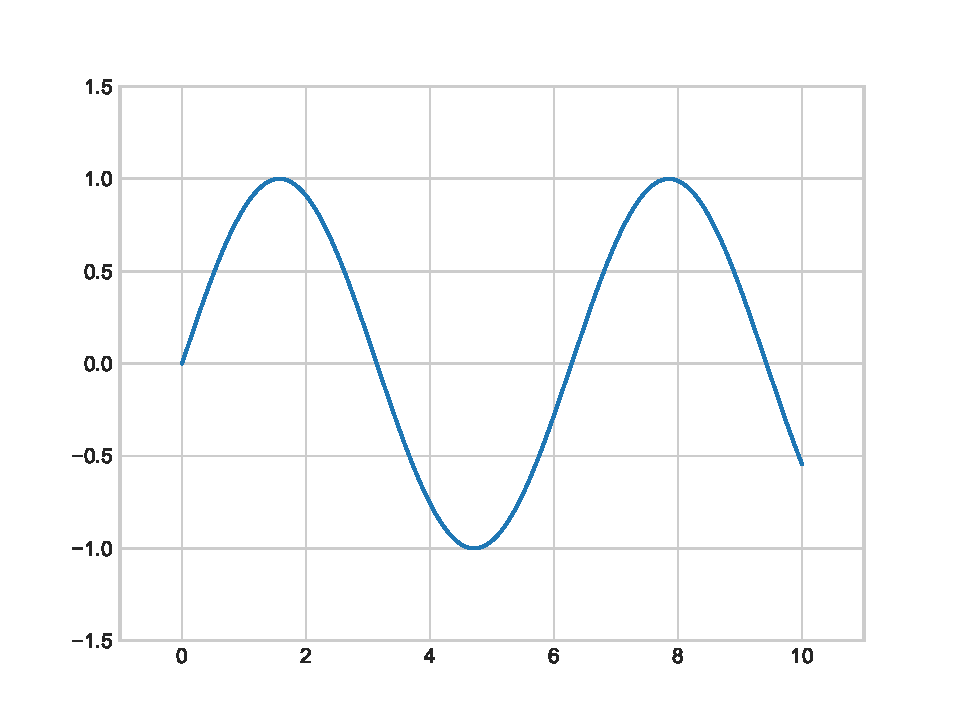
\includegraphics[width=.85\linewidth]{./pics/Figure_8}
	\caption{Пример настройки пределов координатных осей}
	\label{fig:fig_8}
\end{figure}
\end{minipage}
\vfill
\end{frame}

\begin{frame}[fragile, label=m]{Пределы осей координат}
\scriptsize
Альтернативный способ~-- вызов метода \texttt{plt.axis()}. Данный метод дает возможность задавать пределы значений координатных осей путем передачи списка \texttt{[xmin, xmax, ymin, ymax]} (рисунок~\ref{fig:fig_9}):
\vfill
\begin{minipage}{.4\textwidth}
\begin{minted}{python}
import numpy as np
import matplotlib.pyplot as plt


plt.style.use('seaborn-v0_8-whitegrid')

x = np.linspace(0, 10, 1000)
plt.plot(x, np.sin(x))
plt.axis([0, 5, -1.1, 1.1])

plt.show()
|\space|
\end{minted}
\end{minipage}
\begin{minipage}{.59\textwidth}
\begin{figure}[h!]
	\centering
	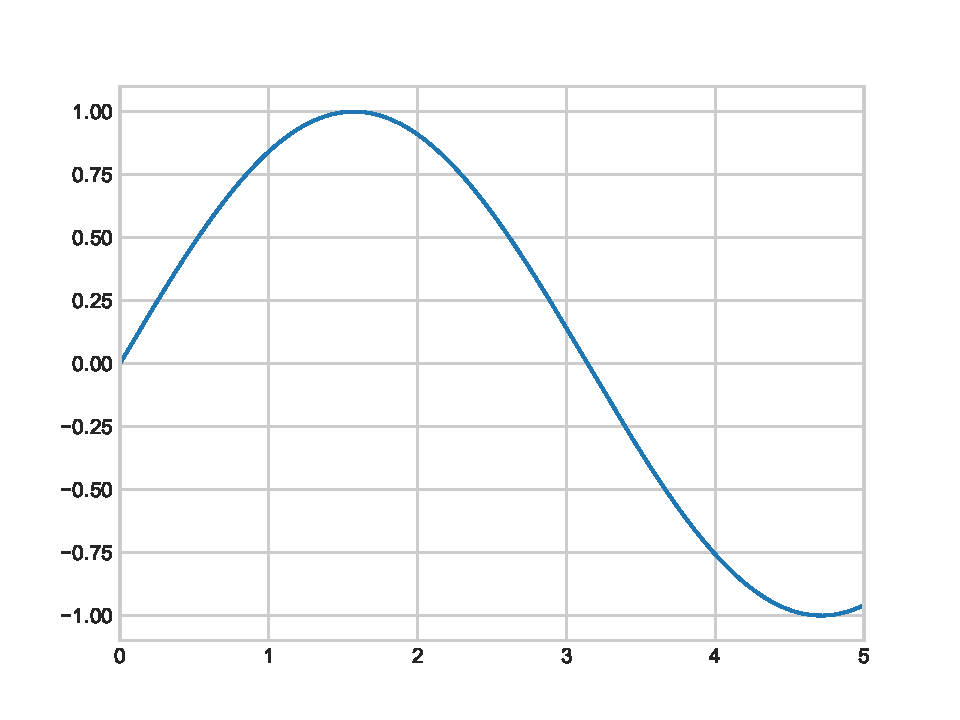
\includegraphics[width=.85\linewidth]{./pics/Figure_9}
	\caption{Настройка пределов координатных осей посредством метода \texttt{plt.axis()}}
	\label{fig:fig_9}
\end{figure}
\end{minipage}
\vfill
\end{frame}

\subsection{Метки на графиках}
\begin{frame}[fragile, label=m]{Метки на графиках}
\scriptsize
Для быстрого определения названий и меток осей существуют специальные методы (рисунок \ref{fig:fig_11}):
\vfill
\begin{minipage}{.4\textwidth}
\begin{minted}{python}
import numpy as np
import matplotlib.pyplot as plt


plt.style.use('seaborn-v0_8-whitegrid')

x = np.linspace(0, 10, 1000)
plt.plot(x, np.cos(x))

# График функции y = cos(x)
plt.title('График функции y = cos(x)')
plt.xlabel('x')
plt.ylabel('cos(x)')

plt.show()
|\space|
\end{minted}
\end{minipage}
\begin{minipage}{.59\textwidth}
\begin{figure}[h!]
	\centering
	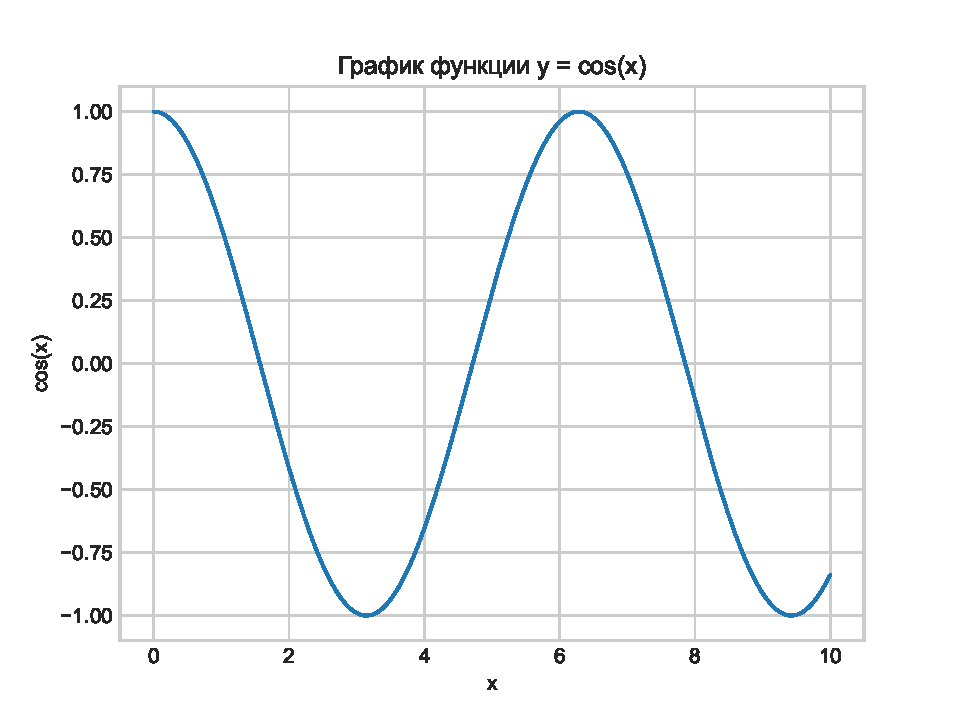
\includegraphics[width=.85\linewidth]{./pics/Figure_11}
	\caption{Пример настройки заголовка графика и названий осей координат}
	\label{fig:fig_11}
\end{figure}
\end{minipage}
\vfill
\end{frame}

\subsection{Метки на графиках}
\begin{frame}[fragile, label=m]{Метки на графиках}
\scriptsize
Когда требуется отобразить несколько линий в одной координатной сетке, часто бывает необходимо создать легенду, на которой была бы отмечена каждая линия. Для быстрого решения данной задачи в Matplotlib есть метод \texttt{plt.legend()} (рисунок~\ref{fig:fig_12}):
\vfill
\begin{minipage}{.4\textwidth}
\begin{minted}{python}
import numpy as np
import matplotlib.pyplot as plt


plt.style.use('seaborn-v0_8-whitegrid')

x = np.linspace(0, 10, 1000)
plt.plot(x, np.cos(x), color='b',
         linestyle='-',
         label='cos(x)')
plt.plot(x, np.sin(x), color='g',
         linestyle=':',
         label='sin(x)')

plt.legend()
plt.show()
|\space|
\end{minted}
\end{minipage}
\begin{minipage}{.59\textwidth}
\begin{figure}[h!]
	\centering
	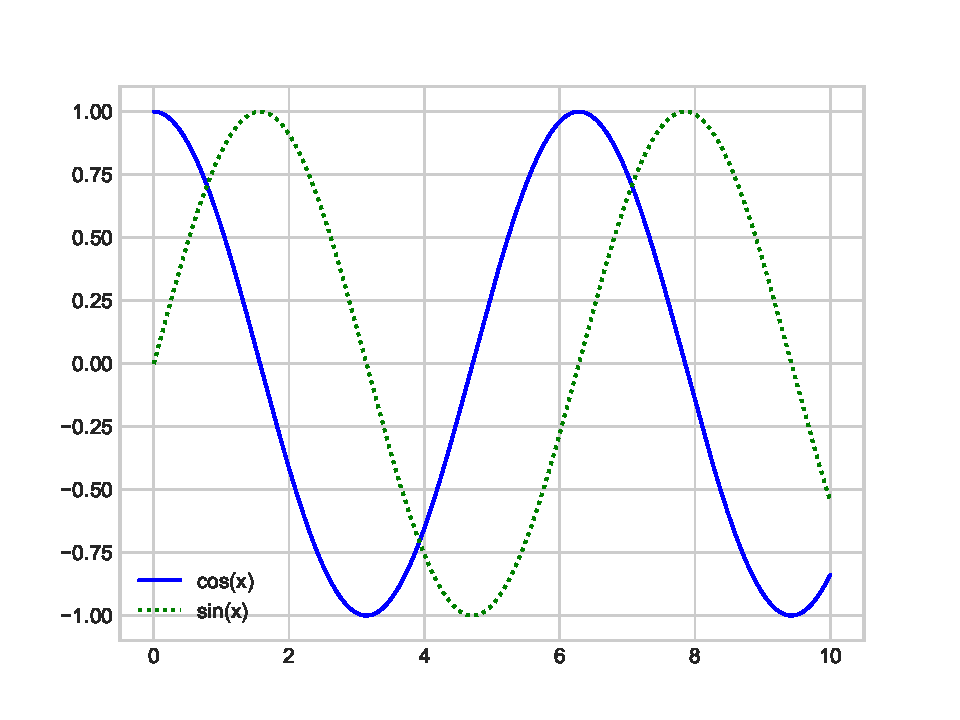
\includegraphics[width=.85\linewidth]{./pics/Figure_12}
	\caption{Пример настройки легенды графика с помощью метода \texttt{plt.legend()}}
	\label{fig:fig_12}
\end{figure}
\end{minipage}
\vfill
\end{frame}

\subsection{Диаграммы рассеяния}
\begin{frame}[fragile, label=m]{Диаграммы рассеяния}
\scriptsize
Наряду с линейными графиками, еще одним распространенным типом является диаграмма рассеяния. В таких диаграммах точки не соединяются линиями, а представляются отдельно (рисунок~\ref{fig:fig_13}):
\vfill
\begin{minipage}{.4\textwidth}
\begin{minted}{python}
import numpy as np
import matplotlib.pyplot as plt


plt.style.use('seaborn-v0_8-whitegrid')

x = np.linspace(0, 10, 30)
y = np.sin(x)

plt.plot(x, y, 'o', color='black')
plt.show()
|\space|
\end{minted}
\end{minipage}
\begin{minipage}{.59\textwidth}
\begin{figure}[h!]
	\centering
	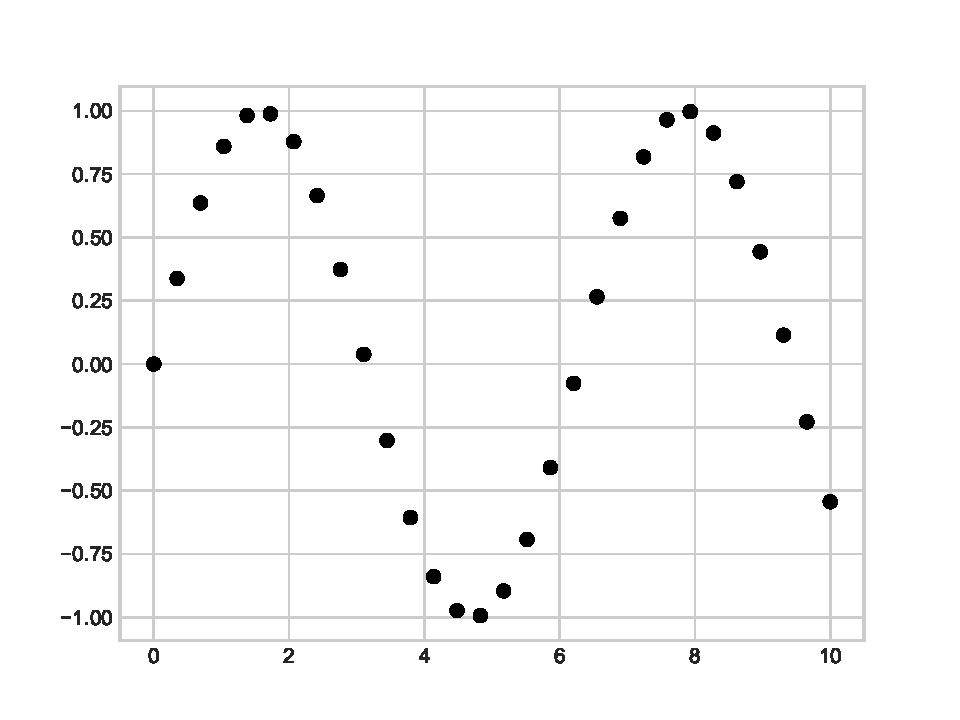
\includegraphics[width=.85\linewidth]{./pics/Figure_13}
	\caption{Пример построения диаграммы рассеяния с помощью функции \texttt{plt.plot()}}
	\label{fig:fig_13}
\end{figure}
\end{minipage}
\vfill
\end{frame}

\begin{frame}[fragile, label=m]{Диаграммы рассеяния}
\scriptsize
Третий аргумент в вызове \texttt{plt.plot()} задает тип символа, используемого при построении графика. Для стилей маркеров существует собственный набор сокращенных строковых кодов (рисунок~\ref{fig:fig_14}):
\vfill
\begin{minted}{python}
import numpy as np
import matplotlib.pyplot as plt


plt.style.use('tableau-colorblind10')

rng = np.random.RandomState(0)
for marker in ['o', '.', ',', 'x', '+', 'v', '^',
               '<', '>', 's', 'd']:
    plt.plot(rng.rand(5), rng.rand(5), marker,
             label=f"marker='{marker}'")

plt.legend()
plt.xlim(0, 1.8)

plt.show()
|\space|
\end{minted}
\vfill
\end{frame}

\begin{frame}[fragile, label=m]{Диаграммы рассеяния}
\scriptsize
\begin{figure}[h!]
	\centering
	
\includegraphics[width=.69\linewidth]{./pics/Figure_14}
	\caption{Пример использования строковых кодов для маркеров диаграммы рассеяния}
	\label{fig:fig_14}
\end{figure}
\vfill
\end{frame}

\begin{frame}[fragile, label=m]{Диаграммы рассеяния}
\scriptsize
Символьные коды для маркеров разрешено использовать совместно с кодами линий и цветов, отображая на графике точки вместе с соединяющими их линиями (рисунок~\ref{fig:fig_15}):
\begin{minipage}{.4\textwidth}
\begin{minted}{python}
import numpy as np
import matplotlib.pyplot as plt


plt.style.use('seaborn-v0_8-whitegrid')

x = np.linspace(0, 10, 30)
y = np.sin(x)

# штриховая линия (--),
# маркер ромба (d) черный цвет (k)
plt.plot(x, y, '--dk')
plt.show()
|\space|
\end{minted}
\end{minipage}
\begin{minipage}{.59\textwidth}
\begin{figure}[h!]
	\centering
	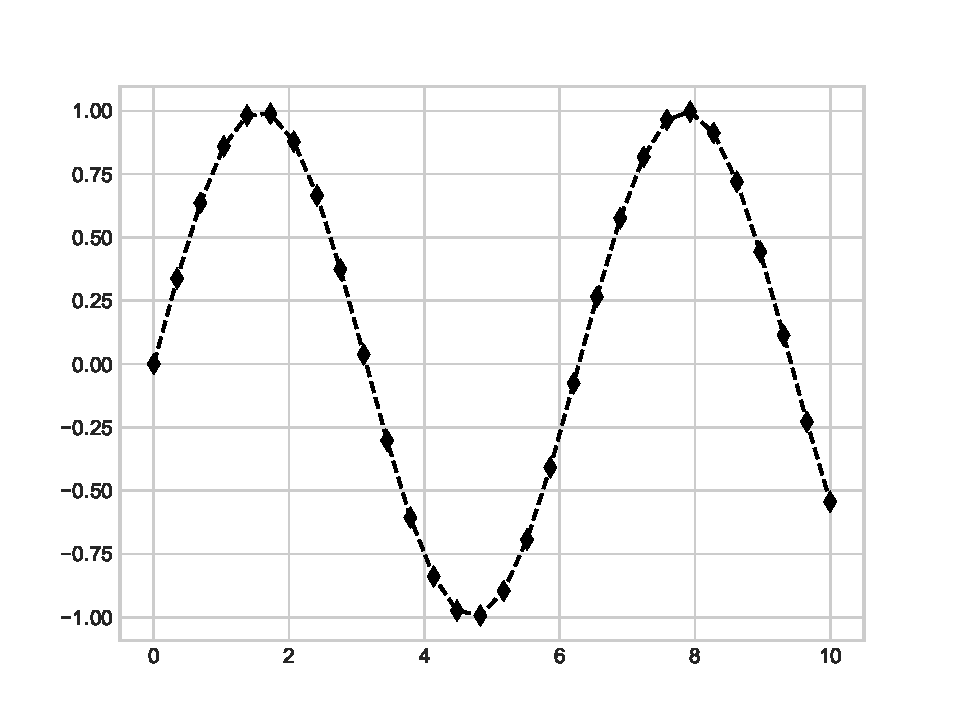
\includegraphics[width=.85\linewidth]{./pics/Figure_15}
	\caption{Пример сочетания линий и маркеров точек}
	\label{fig:fig_15}
\end{figure}
\end{minipage}
\vfill
\end{frame}

\begin{frame}[fragile, label=m]{Диаграммы рассеяния}
\scriptsize
Используя дополнительные ключевые аргументы функции \texttt{plt.plot()} можно определять множество свойств линий и маркеров (рисунок~\ref{fig:fig_16}):
\vfill
\begin{minipage}{.4\textwidth}
\begin{minted}{python}
import numpy as np
import matplotlib.pyplot as plt


plt.style.use('seaborn-v0_8-whitegrid')

x = np.linspace(0, 10, 30)
y = np.sin(x)

plt.plot(x, y, '-p', color='gray',
         markersize=14, linewidth=4,
         markerfacecolor='white',
         markeredgecolor='gray',
         markeredgewidth=1)
plt.ylim(-1.2, 1.2)

plt.show()
|\space|
\end{minted}
\end{minipage}
\begin{minipage}{.59\textwidth}
\begin{figure}[h!]
	\centering
	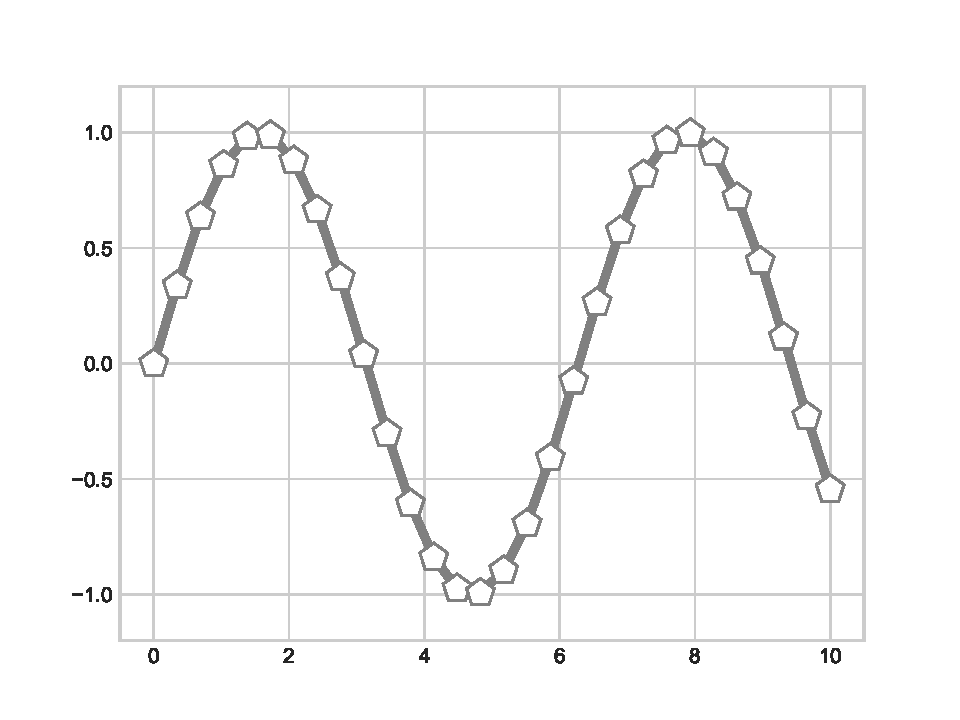
\includegraphics[width=.85\linewidth]{./pics/Figure_16}
	\caption{Пример индивидуальной настройки вида линий и маркеров точек}
	\label{fig:fig_16}
\end{figure}
\end{minipage}
\vfill
\end{frame}

\begin{frame}[fragile, label=m]{Диаграммы рассеяния}
\scriptsize
Функция построения диаграмм \texttt{plt.scatter()}, в многом похожая на  \texttt{plt.plot()}, обладает еще более расширенными возможностями (рисунок~\ref{fig:fig_17}):
\vfill
\begin{minipage}{.4\textwidth}
\begin{minted}{python}
import numpy as np
import matplotlib.pyplot as plt


plt.style.use('seaborn-v0_8-whitegrid')

x = np.linspace(0, 10, 30)
y = np.sin(x)

plt.scatter(x, y, marker='o')

plt.show()
|\space|
\end{minted}
\end{minipage}
\begin{minipage}{.59\textwidth}
\begin{figure}[h!]
	\centering
	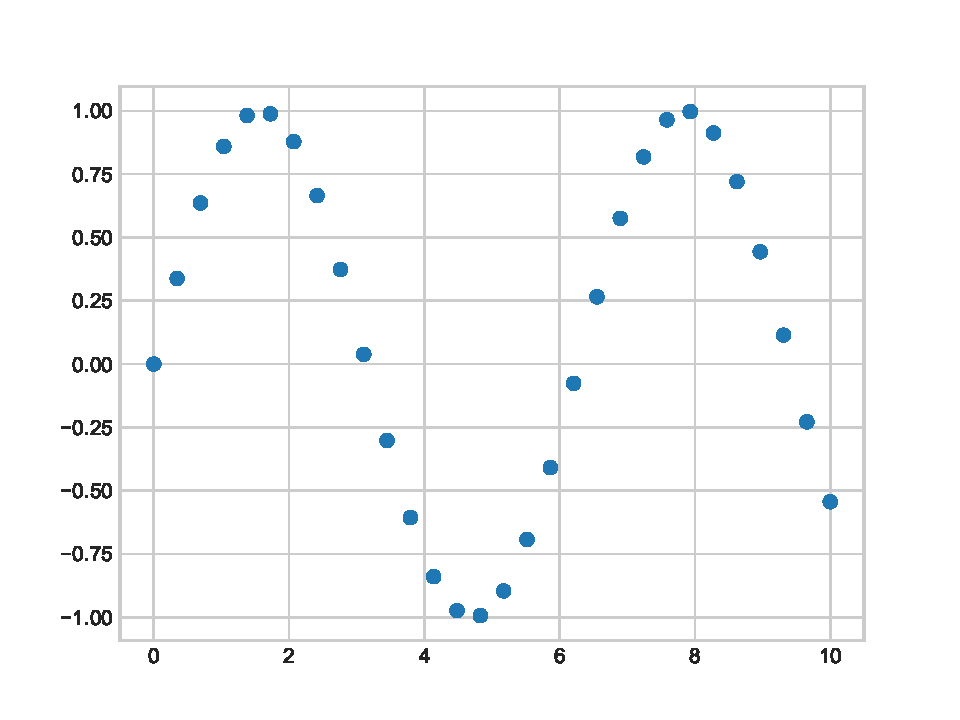
\includegraphics[width=.85\linewidth]{./pics/Figure_17}
	\caption{Диаграмма рассеяния, построенная с использованием метода \texttt{plt.scatter()}}
	\label{fig:fig_17}
\end{figure}
\end{minipage}
\vfill
\end{frame}

\begin{frame}[fragile, label=m]{Диаграммы рассеяния}
\scriptsize
При помощи \texttt{plt.scatter()} можно создавать диаграммы рассеяния с индивидуальными свойствами каждой точки (такими как размер, заливка, цвет рамки и т.д.).

Создадим случайную диаграмму рассеяния с точками различных размеров и цветов. Воспользуемся ключевым аргументом \texttt{alpha}, отвечающим за уровень прозрачности (рисунок \ref{fig:fig_18}):
\vfill
\begin{minipage}{.4\textwidth}
\begin{minted}{python}
import numpy as np
import matplotlib.pyplot as plt
rng = np.random.RandomState(0)

x = rng.randn(100)
y = rng.randn(100)
colors = rng.rand(100)
sizes = 1000 * rng.rand(100)
plt.scatter(x, y, c=colors,
            s=sizes, alpha=0.3,
            cmap='viridis')
plt.colorbar()  # цветовая шкала
plt.show()
|\space|
\end{minted}
\end{minipage}
\begin{minipage}{.59\textwidth}
\begin{figure}[h!]
	\centering
	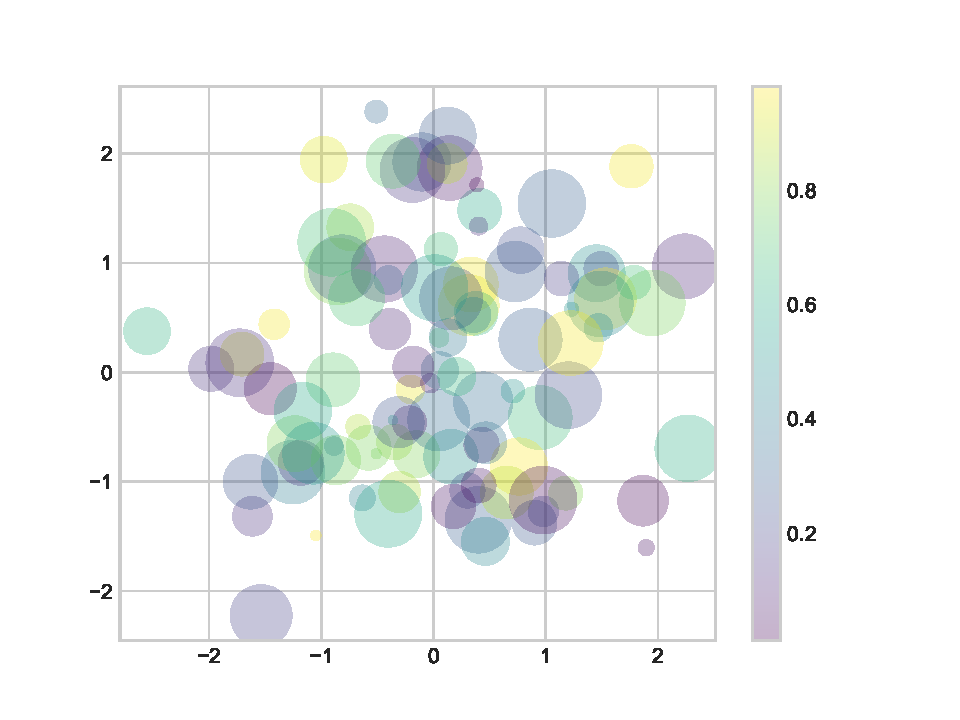
\includegraphics[width=.73\linewidth]{./pics/Figure_18}
	\caption{Настройка размера, цвета и прозрачности точек диаграммы рассеяния при помощи функции \texttt{plt.scatter()}}
	\label{fig:fig_18}
\end{figure}
\end{minipage}
\vfill
\end{frame}

\subsection{Гистограммы}
\begin{frame}[fragile, label=m]{Гистограммы}
\scriptsize
Функция \texttt{hist()} поддерживает множество параметров для настройки вычисления и отображения. Рассмотрим пример гистограммы с детальными пользовательскими настройками (рисунок~\ref{fig:fig_20}):
\vfill
\begin{minipage}{.4\textwidth}
\begin{minted}{python}
import numpy as np
import matplotlib.pyplot as plt


plt.style.use('seaborn-v0_8-white')
data = np.random.randn(1000)

plt.hist(data, bins=30, alpha=0.5,
         color='steelblue',
         edgecolor='none')

plt.show()
|\space|
\end{minted}
\end{minipage}
\begin{minipage}{.59\textwidth}
\begin{figure}[h!]
	\centering
	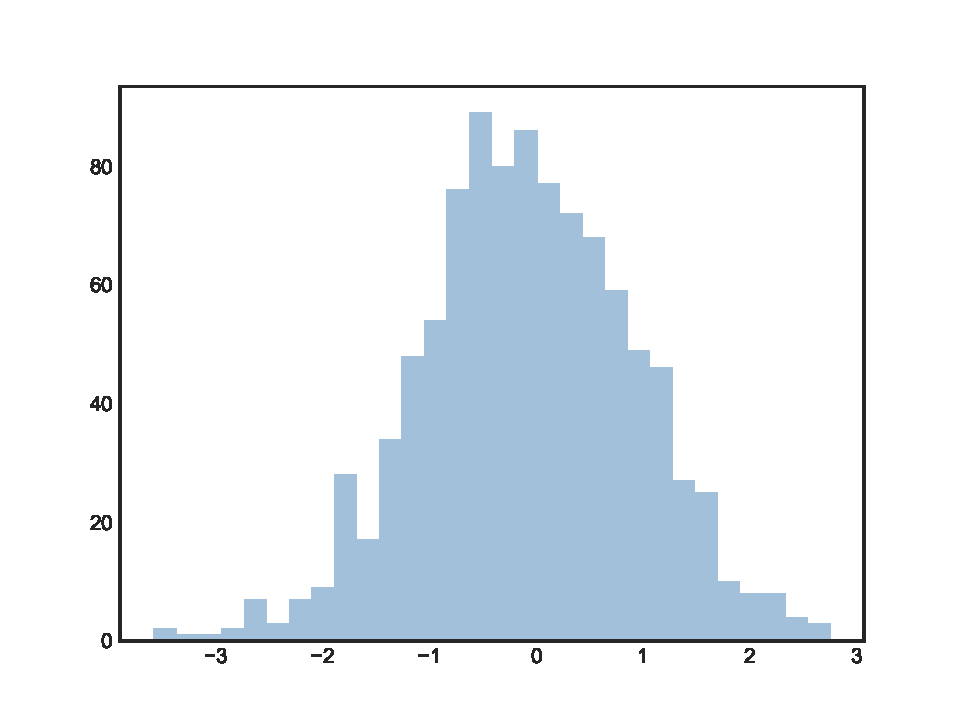
\includegraphics[width=.85\linewidth]{./pics/Figure_20}
	\caption{Пример гистограммы с пользовательскими настройками}
	\label{fig:fig_20}
\end{figure}
\end{minipage}
\vfill
\end{frame}

\begin{frame}[fragile, label=m]{Гистограммы}
\scriptsize
Сравнение гистограмм нескольких распределений (рисунок~\ref{fig:fig_21}):
\vfill
\begin{minipage}{.4\textwidth}
\begin{minted}{python}
import numpy as np
import matplotlib.pyplot as plt


x1 = np.random.normal(0, 0.8, 1000)
x2 = np.random.normal(-2, 1, 1000)
x3 = np.random.normal(3, 2, 1000)

options = dict(alpha=0.3, bins=40)

plt.hist(x1, **options)
plt.hist(x2, **options)
plt.hist(x3, **options)

plt.show()
|\space|
\end{minted}
\end{minipage}
\begin{minipage}{.59\textwidth}
\begin{figure}[h!]
	\centering
	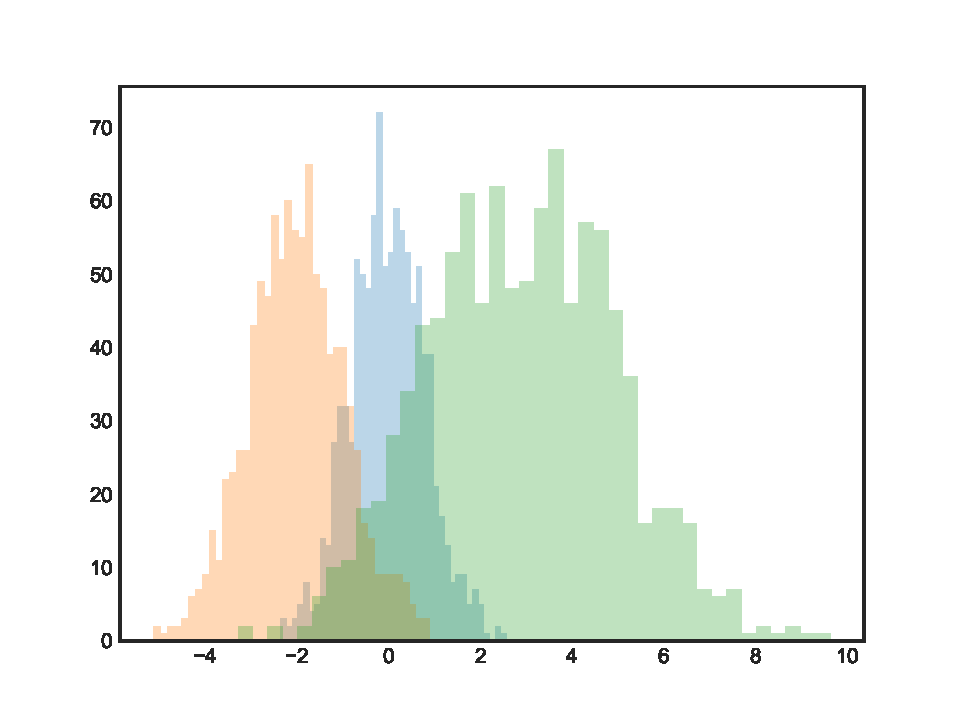
\includegraphics[width=.9\linewidth]{./pics/Figure_21}
	\caption{Несколько гистограмм с наложением}
	\label{fig:fig_21}
\end{figure}
\end{minipage}
\vfill
\end{frame}

\subsection{Трехмерные графики}
\begin{frame}[fragile, label=m]{Трехмерные графики}
\scriptsize
Модуль \texttt{mplot3d} содержит инструменты для отображения трехмерных графиков. Функция \texttt{ax.contour3D()} ожидает данные в формате двумерных регулярных сеток (рисунок~\ref{fig:fig_24}):
\vfill
\begin{minipage}{.4\textwidth}
\begin{minted}{python}
import numpy as np
import matplotlib.pyplot as plt

def fun(x, y):
    return np.sin(np.sqrt(x ** 2 + y ** 2))

x = np.linspace(-6, 6, 30)
y = np.linspace(-6, 6, 30)
x_mesh, y_mesh = np.meshgrid(x, y)
z_mesh = fun(x_mesh, y_mesh)

fig = plt.figure()
ax = plt.axes(projection='3d')
ax.contour3D(x_mesh, y_mesh, z_mesh,
             50, cmap='cool')
ax.set_xlabel('x')
ax.set_ylabel('y')
ax.set_zlabel('z')
plt.show()
\end{minted}
\end{minipage}
\begin{minipage}{.09\textwidth}
\hfill
\end{minipage}
\begin{minipage}{.5\textwidth}
\begin{figure}[h!]
	\centering
	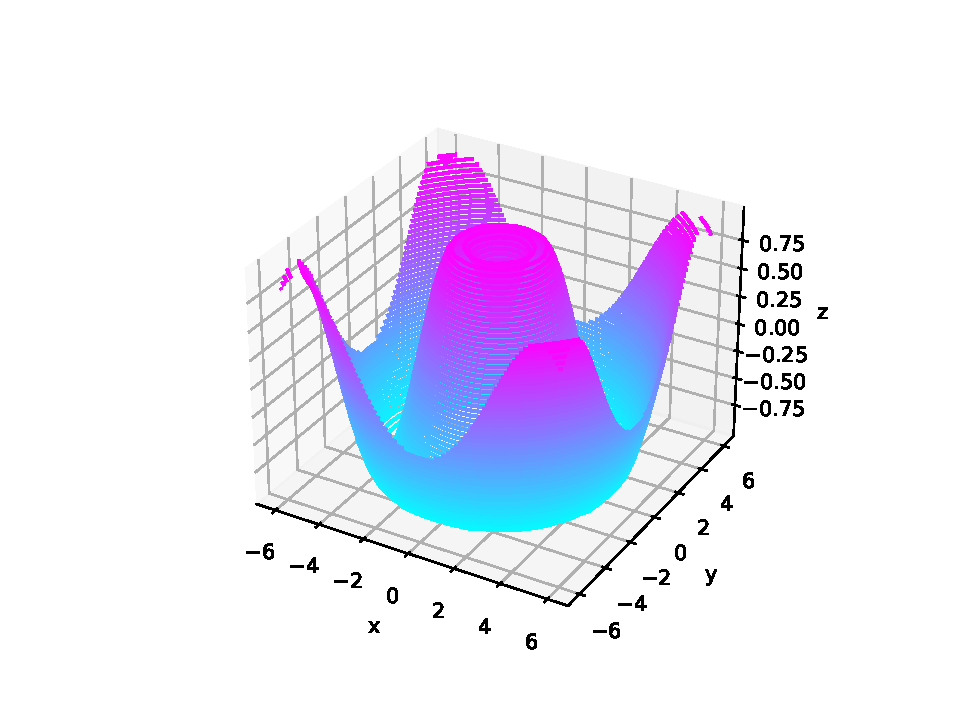
\includegraphics[width=.87\linewidth]{./pics/Figure_24}
	\caption{Построение трехмерного графика при помощи функции \texttt{ax.contour-3D()}}
	\label{fig:fig_24}
\end{figure}
\end{minipage}
\vfill
\end{frame}

\begin{frame}[fragile, label=m]{Трехмерные графики}
\scriptsize
Для изменения угла возвышения нужно применить метод \mintinline{python}|view_init|. Для примера, приведенного на рисунке \ref{fig:fig_24} можно выбрать следующие параметры: угол возвышения $60$ градусов (т.е. $60$ градусов над плоскостью $X$-$Y$); азимут $35$ градусов (т.е. график будет повернут на $35$ градусов против часовой стрелки вокруг оси $Z$):
\vfill
\begin{minipage}{.4\textwidth}
\begin{minted}[firstnumber=last]{python}
|\space|
|\space|
fig = plt.figure()
ax = plt.axes(projection='3d')
ax.contour3D(x_mesh, y_mesh, z_mesh,
             50, cmap='cool')
ax.set_xlabel('x')
ax.set_ylabel('y')
ax.set_zlabel('z')
ax.view_init(60, 35)
plt.show()
|\space|
\end{minted}
\end{minipage}
\begin{minipage}{.09\textwidth}
\hfill
\end{minipage}
\begin{minipage}{.5\textwidth}
\begin{figure}[h!]
	\centering
	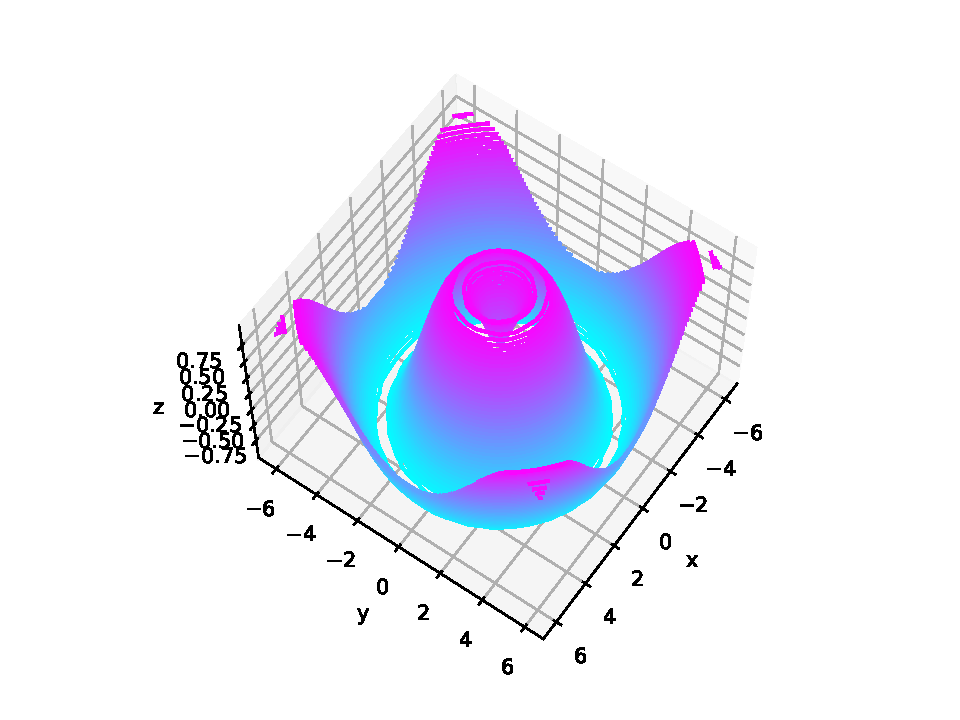
\includegraphics[width=.8\linewidth]{./pics/Figure_25}
	\caption{Настройка угла зрения для трехмерного графика}
	\label{fig:fig_25}
\end{figure}
\end{minipage}
\vfill
\end{frame}

\contactsframe[\Large \textbf{Благодарю за внимание!}]{

\bigskip

\includegraphics[width=.05\textwidth]{pics/home} \quad Учебный корпус №2, ауд. 136 \\

\includegraphics[width=.05\textwidth]{pics/mail} \quad chuva@tpu.ru \\

\includegraphics[width=.03\textwidth]{pics/tel} \quad +7-962-782-66-15
}

\end{document}

